% Kota Miura (miura at embl.de)
% Macro Course Textbook 

\documentclass[11pt,a4paper,oneside]{report}
% Palatino for rm and math | Helvetica for ss | Courier for tt
\usepackage{mathpazo} % math & rm
\linespread{1.05}        % Palatino needs more leading (space between lines)
\usepackage[scaled]{helvet} % ss
\usepackage{courier} % tt
%\usepackage{inconsolata} %tt
%\usepackage[scaled]{ulgothic} %tt no style fi
%\renewcommand*\ttdefault{cmvtt} %tt
%\renewcommand*\ttdefault{lmvtt} %tt OK

\normalfont
\usepackage[T1]{fontenc}
\usepackage[footnotesize]{caption}
\usepackage{subfig}

\linespread{1.05}         % Palatino needs more leading (space between lines)
\usepackage{hyperref}
\hypersetup{colorlinks=true, linkcolor=blue, urlcolor=blue}

%\usepackage{url} % this will just show url in different font
\usepackage[pdftex]{graphicx}
\usepackage{color}
\definecolor{gray09}{rgb}{0.9,0.9,0.9}  %background for codes
\definecolor{red}{rgb}{1,0,0}
\definecolor{blue}{rgb}{0,0,1}
\definecolor{lightblue}{rgb}{0,0.8,1}

%for header
\usepackage{fancyhdr}
\setlength{\headheight}{15.2pt}
%\pagestyle{fancy}
\pagestyle{fancyplain}
\renewcommand{\chaptermark}[1]{\markboth{#1}{}}
\renewcommand{\sectionmark}[1]{\markright{\thesection\ #1}{}}
 
\lhead{\fancyplain{}{\textit{CMCI ImageJ Macro Course}}}
\chead{}
\rhead{\fancyplain{}{\textit{\rightmark}}}
\lfoot{}
\cfoot{\fancyplain{}{\thepage}}
\rfoot{}

% space between paragraphs
\parskip 7.2pt

% indent
\setlength{\parindent}{0in} % avoids indent at the beginning of paragraph
 
%%\usepackage{lipsum}
%\newenvironment{indentexercise}[1]%
%{\begin{list}{}%
%         {\setlength{\leftmargin}{#1}}%
%         \item[]%
%}
%{\end{list}}
\newenvironment{indentexercise}[1]%
{{\setlength{\leftmargin}{2em}}%
\textbf{Exercise \thesubsection-#1}%
\begin{list}{}% 
	\item%
}
{\end{list}}

%indenting for case with Fiji
\newenvironment{indentFiji}%
{\begin{list}{}%
         {\setlength{\leftmargin}{1em}}%
         \item[]%
}
{\end{list}}

%indenting for case with Command Definition
\newenvironment{indentCom}%
{\begin{list}{}%
         {\setlength{\leftmargin}{1em}}%
         \item[]%
}
{\end{list}}

%\colorbox{red}

%command for menu tree
\newcommand{\ijmenu}[1]{\texttt{\small#1}}

%command for inline code
\newcommand{\ilcom}[1]{\texttt{\small#1}}

%quick command for making space
 \newcommand{\tab}{\hspace*{3em}}

% packge for codes
% --- source code matters ---
\usepackage{listings}
%\usepackage{listingsutf8}
\lstset{ %
%language=Octave,                % choose the language of the code
%basicstyle=\footnotesize,       % the size of the fonts that are used for the code
basicstyle=\small\ttfamily, % same as above, but use typewriter
numbers=left,                   % where to put the line-numbers
numberstyle=\footnotesize,      % the size of the fonts that are used for the line-numbers
stepnumber=1,                   % the step between two line-numbers. If it's 1 each line 
                                % will be numbered
numbersep=5pt,                  % how far the line-numbers are from the code
backgroundcolor=\color{gray09},  % choose the background color. You must add \usepackage{color}
keywordstyle=\color{blue}, 	%added
showspaces=false,               % show spaces adding particular underscores
showstringspaces=false,         % underline spaces within strings
showtabs=false,                 % show tabs within strings adding particular underscores
%frame=single,                   % adds a frame around the code
%frame=trBL,
tabsize=2,                      % sets default tabsize to 2 spaces
captionpos=b,                   % sets the caption-position to bottom
breaklines=true,                % sets automatic line breaking
%breakatwhitespace=false,        % sets if automatic breaks should only happen at whitespace
title=\lstname,                 % show the filename of files included with \lstinputlisting;
                                % also try caption instead of title
escapeinside={\%*}{*)},         % if you want to add a comment within your code
morekeywords={*,...},            % if you want to add more keywords to the set
morecomment=[l]{//},
morecomment=[s]{/*}{*/},
morestring=[b]",
%aboveskip={7.2pt}	%supposed to be the space above llisting but dows not work. 
%belowskip={7.2pt}
}

\newcommand{\HRule}{\rule{\linewidth}{0.5mm}}

%using eps
\usepackage{epstopdf}

% title page matters
% http://sunsite.bilkent.edu.tr/pub/tex/ctan/info/latex-samples/titlepages.pdf
\newcommand*{\titleTH}{\begingroup% T&H Typography
\raggedleft
\HRule\\
\vspace*{\baselineskip}
{\Large Kota Miura}\\[0.167\textheight]

{\bfseries EMBL-CMCI course II}\\[\baselineskip]
{\textcolor{Medium}{\Huge Macro Programming in ImageJ}}\\[\baselineskip]
{\small ver 2.0.2}\par
\vfill

%{\Large Centre for Molecular \& Cellular Imaging\\EMBL Heidelberg\\\plogo}\par
{\Large Centre for Molecular \& Cellular Imaging\\EMBL Heidelberg}\par

\includegraphics[width=0.15\textwidth]{fig/rgb_logo_2006_win.eps} 

\includegraphics[width=0.07\textwidth]{fig/Icon30pedge.jpg}\\[1cm] 
\vspace*{3\baselineskip}
\HRule\\
\endgroup}

\definecolor{Dark}{gray}{.2}
\definecolor{Medium}{gray}{.6}
\definecolor{Light}{gray}{.8}
\definecolor{shadecolor}{rgb}{0.9, 0.9, 1}
%making 1.5 spaced lines
\usepackage{setspace}
\onehalfspacing

% background shading
\usepackage{framed}

\usepackage{pdfsync}
%%%%%%%%%%%%%%%%%%%%%%%%%

\begin{document}
\title{Image Processing and Analysis Course II\\
Macro Programming in ImageJ}
\author{Kota Miura\\
\\
  Centre for Molecular and Cellular Imaging,\\
  EMBL Heidelberg,\\
  Germany\\
\\
\texttt{miura@embl.de}
}

\date{\today}

%\maketitle
\pagestyle{empty}
\titleTH
\clearpage
\pagestyle{fancyplain}
\begin{abstract}
\HRule
\\
\\
\textbf{Aim: Students acquire ImageJ macro programming technique 
to ease their work loads with image processing / analysis.}
\\
\\
%need to fix greek beta
Note: This textbook was written using Fiji (ImageJ 1.44e). 
When you want to distribute, please ask Kota as this textbook is progressively edited.
\\
Compiled on \today \\
$\copyright$ 2006 - 2012, Kota Miura (http://cmci.embl.de)
\\
\HRule
\end{abstract}

\begingroup
\hypersetup{linkcolor=black}
\tableofcontents
\endgroup

\clearpage
\setcounter{chapter}{2}
\section{Why do we write macro?}

\dots to make your life easier by:

\subsection{Automate your mouse clicking!}

ImageJ commands can be listed in a text file as a sequence of event and then executed as a single task. 
Writing such a text file is called scripting, or writing a ``macro''. 

For example, if you want to do \\
\ijmenu{[Process -> Contrast Enhancement]}, \\
apply \ijmenu{[Process -> Gaussian blurring]} \\
and then \ijmenu{[Process -> threshold]} \\
to an image, it takes three times of mouse operation choosing these commands from ImageJ menu. 
If you need to do this for many images, the work load would become pretty heavy. 
Writing a macro assembles such works into a single task. Macro becomes even more powerful 
when you need to process/analyze stacks. 

\subsection{Generate new functions which do not exist in the menu or as a PlugIn.}
Automation of a series of command is very convenient, 
but the macro programming is not only limited to such automation. 
ImageJ macro language enables you to access single pixels in digital images. 
This means that when you know an algorithm for processing/analysis 
but the function is not implemented in the ImageJ 
itself or as a PlugIn, one could write a custom function using the macro language.
\subsection{Running your job in remote server}
ImageJ could be used from command line, and macro file could be executed by 
adding the file name to the java command. 
This enables you to do the calculation with faster machines like the EMBL cluster. 
If you use job array many jobs could be done in parallel so you could finish your calculation much faster.

\subsection{Limitations compared to Plugins written in Java}

In addition to Macro programming, ImageJ has plugin-writing capability. 
This enables one to add new functions to ImageJ by coding in Java programming language. 
This capability affords almost infinite possibility to process and analyze images; 
you could create any kind of processing / analysis functions you could imagine. 
Compared to plugins, ImageJ Macro language has some limitations: 

\begin{enumerate}
\item If you need to process large images or stacks with many steps, 
you might recognize that it is slow. 
Some benchmarks indicates that a Plugin would be about 40 times faster than Macro. 

\item Macro cannot be used as a library
\footnote{It is possible to write a macro in a library fashion and use it from another macro, 
but this is not as robust and clear as it is in java, which is a language designed to be so.}. 
In Java, once a class is written, this could be used later again from another class . 

\item Macro is not efficient in implementing real-time interactive input 
during the macro command is executed; 
\textit{e.g.} If you want to design a program that requires real-time user input 
to select a ROI interactively.  
Macro could only do such interactive tasks by separating the program into several different commands. 
\end{enumerate}

If you become unsatisfied with these limitations, 
learning more complicated but more flexible PlugIn programming is recommended. 

\subsection{Comparison with Other scripting languages}
There are several other scripting capability for customizing ImageJ function. 
This is because ImageJ is a java program, 
and there are many scripting languages that are interfaced with Java. 
Scripting languages included in Fiji are 

\begin{itemize}
 \item Javascript
 \item Jython (Java-Python)
 \item JRuby (Java-Ruby)
 \item Clojure
 \end{itemize}

If you set up environment by yourself, you could also use other languages such as Scala and Groovy. 
Compared to ImageJ macro language, all these languages are more general and widely used. 

Advantages of ImageJ Macro compared to these scripting languages are: 
\begin{itemize}
\item Easy to learn. 
Functions are mirrors of ImageJ menu, so scripting is intuitive if you know ImageJ already. 
Macro recorder is a handy tool for finding out the right commands. 

\item Macro set allows you to contain multiple macros in one file (called 'Macro-set"). 
This is useful for complex processing is required (see Advanced Macro Programming section for more details). 

\item A significant hurdle for coding with general scripting languages is that one must know the 
\textbf{ImageJ Java API} well, meaning that you basically have to know 
fundamentals of Java programming language 
for using these scripting languages. 
\end{itemize}

Thus, ImageJ macro language is the easiest way to access scripting capability in ImageJ. 

Disadvantage of ImageJ macro compared to other scripting languages 
beside its generality is its extendability: 
code you write could not be recycled except with copy and pasting
\footnote{One could also use getArgument() and File related functions for passing arguments 
from a macro file to the other, but ImageJ macro is not designed to be a library. }. 
With other scripting languages available for ImageJ, one could write more object-oriented programs 
and once you write, code could be recycled in other programs
\footnote{ Except for Javascript. Calling other Javascript 
file from another Javascript file is not straight forward.}. 
Another disadvantage is that Macro is slow compared to some of scripting languages like Clojure and Scala. 
Processing speed is comparable to Jython and Javascript.  

\subsection{Summary}
Macro programming enables you to ease the work loads by automating sequence of commands. 
Accessing single pixels from macro is also possible. 
The potential of the macro is similar to PlugIn, but for interactive functions PlugIn works better. 
Macro is also slower than plugin. 

\textbf{How to learn Macro programming:} 
In this course, you will encounter with many example codes. 
You will write the example codes in your own laptop ImageJ and run the macro. 
Modifying these examples is a very important exercise since in most cases, 
you start writing your macro by modifying some parts of the macro that is distributed already
\footnote{200+ macros are available in ImageJ web site. 
\href{http://rsb.info.nih.gov/ij/macros/}{http://rsb.info.nih.gov/ij/macros/}}. 
\newpage
\section{Basics}

\subsection{''Hello World!''}

We first try writing a simple macro that prints out''Hello World!''. 
ImageJ has a macro editor with simple debugger function
\footnote{Debugger assists you to correct mistakes in the code. 
This is convenient when the code becomes long. 
Macro can be written in any text editor such as "Notepad" in Windows but of course 
there is no debugger function available in this case.}. 
To open the editor, select \ijmenu{[PlugIns -> New -> Macro]} from the menu.  
This will create a new window where you can write macro (we call this ''macro editor''). 
\begin{indentFiji}
Fiji: You could use more advanced interface called ''script editor'' 
by \ijmenu{[Plugins -> Scripting -> Script Editor]}. 
Then select \ijmenu{[Language -> ImageJ Macro]}. 
Syntax high lighter offers automatic coloring of ImageJ functions. 
\end{indentFiji}
Then write a program as follows
\footnote{NOTE: DON'T FORGET TO TABULATE THE SECOND LINE!}. 
Omit the line numbers! These numbers were added just for explanation. 

%Code 1
%\begin{lstlisting}
%macro "print_out" {
%	print("Hello World!");
%}
%\end{lstlisting}
\lstinputlisting{code/code01.ijm}
%\lstinputlisting[language=Java]{code/code01.ijm}


\begin{figure}[htbp]
\begin{center}
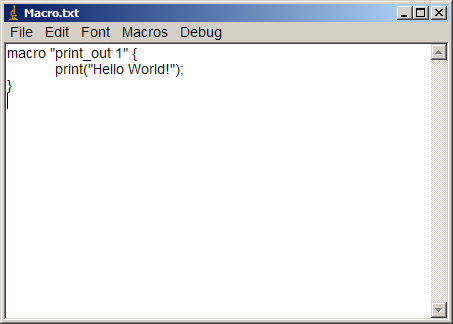
\includegraphics[scale=0.6]{fig/editor_helloworld_IJ.png}
\caption{Macro Editor of ImageJ} \label{fig_MacroEditor}
\end{center}
\end{figure}

\begin{figure}[htbp]
\begin{center}
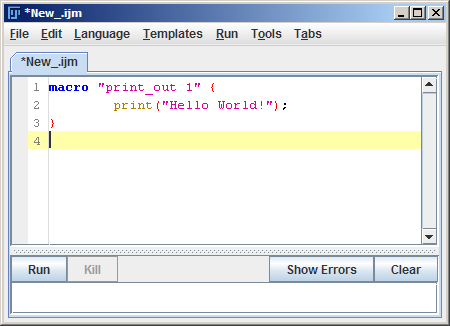
\includegraphics[scale=0.6]{fig/editor_helloworld_fiji.png}
\caption{Script Editor of Fiji} \label{fig_ScriptEditor}
\end{center}
\end{figure}

Click "Macros" in the menu at the top of the macro editing window 
("Macros" in the menu appears only when the macro editing window is active). 
In the first line, there is "Run Macro". 
Try running it from editor menu \ijmenu{[Macros-> Run Macro]} 
\begin{indentFiji}
Fiji:  Use \ijmenu{[Run -> Run]}. 
\end{indentFiji}
This will create a new window "Log", with "Hello World" printed. 

\begin{figure}[htbp]
\begin{center}
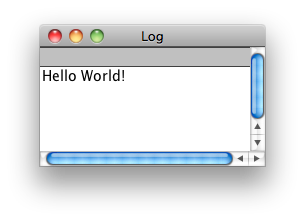
\includegraphics[scale=0.6]{fig/Log_HelloWorld.png}
\caption{Output in Log Window for Code 1} \label{fig23-1}
\end{center}
\end{figure}

Explanation for the Code 1:\\
\begin{itemize}
\item line 1: You are declaring that a macro code starts and the code is contained between 
curly braces \{\}. "print\_out" will be the name of macro. 

\item line2: print() command orders ImageJ to print out the content within the parenthesis 
in the "Log" window. The text to be printed must be contained within the double quotes (""). 
The best reference to macro functions of ImageJ is in the ImageJ web site
\footnote{ http://rsbweb.nih.gov/ij/developer/macro/functions.html}. 
For example, you could find definition of print("") command in the web site as quoted in below:\\
%\item
\begin{indentCom}
\textbf{print(string)}\\
Outputs a string to the "Log" window. Numeric arguments are automatically converted to strings. 
The print() function accepts multiple arguments. For example, you can use print(x,y,width, height) 
instead of print(x+" "+y+" "+width+" "+height). 
If the first argument is a file handle returned by File.open(path), 
then the second is saved in the referred file (see SaveTextFileDemo).

Numeric expressions are automatically converted to strings using four decimal places, 
or use the d2s function to specify the decimal places. 
For example, print(2/3) outputs "0.6667" but print(d2s(2/3,1)) outputs "0.7".
\end{indentCom}

\item line 3: a brace tells ImageJ that the code "print\_out" finishes at this line.  
\end{itemize}
So that was the very basic of how you use a macro. To integrate the macro into the ImageJ Menu bar, 
the macro must be "installed". To do so, in the editor menu, \ijmenu{[Macros -> Install Macros]} 
\begin{indentFiji}
Fiji: [Run -> Install Macro]).
\end{indentFiji}
Check IJ menu \ijmenu{[Macros -> ]} to see that the macro is now in the menu.\\

\begin{figure}[htbp]
\begin{center}
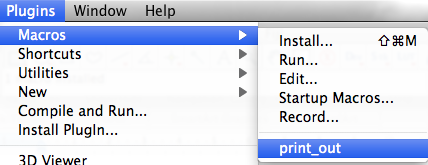
\includegraphics[scale=0.6]{fig/firstMacroInMenu.png}
\caption{Macro Now in ImageJ menu} \label{fig_MacroInMenu}
\end{center}
\end{figure}

Macro can be saved as a file and can be directly installed also. 
In the editor, do \ijmenu{[File -> Save]}. Saving dialogue window appears, 
and just save the file wherever you can remember afterwards . 
To install the macro, do \ijmenu{[PlugIns -> Macro -> Install\ldots]} 
Select the macro file you want to install.\\

%\begin{indentexercise}{1cm}
\begin{indentexercise}{1}
\item Add another line \texttt{"print("\textbackslash{}\textbackslash{}Clear");"} 
after the second line (below, code 1.5. don't forget the semi-colon at the end!). 
\item \lstinputlisting{code/code01_5.ijm}
Then test also another macro when you insert the same command in the third line (code 1.75). 
What happened?  
\item \lstinputlisting{code/code01_75.ijm}
\end{indentexercise}

\begin{indentexercise}{2}
\item Try modifying the third line in code 1.5 
and check that the modified text will be printed in the "Log" window. \\
\end{indentexercise}

\begin{indentexercise}{3}
\item Multiple macros can exist in a single file. We call this \textbf{"macro sets"}. 
Duplicate the code you wrote by copying and pasting under the original. 
The second macro should have a different name. In the example below, the second macro is named "pirnt\_out2".
\end{indentexercise}

\begin{figure}[htbp]
\begin{center}
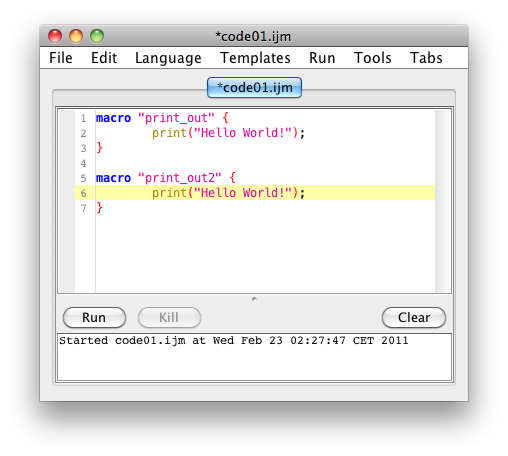
\includegraphics[scale=0.6]{fig/editor_MacroSet.png}
\caption{Macro Set} \label{fig_MacroSetInMenu}
\end{center}
\end{figure}

\subsection{Variables and Strings}
Texts such as "Hello World!" can substituted by variables 
(there is no distinction of number variable and string variable in ImageJ macro.). 
Let's understand this by examining a short macro below.
\lstinputlisting{code/code02.ijm}
\lstinputlisting{code/code03.ijm}

\begin{indentexercise}{1}
\item Add more string variables and make a longer sentence.\\
\end{indentexercise}

Message\_text is a "String Variable" or simply a "String". 
ImageJ prepares a memory space for this variable, and you can change the content by re-defining the content. 
It is also possible to substitute the content with numbers, such as\\
\begin{lstlisting}[numbers=none]
message_text = 256;
\end{lstlisting}
With this assignment, the variable is now a "Numerical variable" or simply "variable". 
In other programming languages such as C or Java, difference between numbers and characters matters a lot. 
In ImageJ you do not have to care whether the variable is number or string, 
but in some cases this may cause problem 
so it's better to just keep this difference in your mind. We will see an example of such confusion, 
and also a way to avoid the confusion. 

Test the following macro to see how the numerical variable works. 
\lstinputlisting{code/code04.ijm}
Did you get some results printed out? It should, but you should read the code carefully. 

You might have noticed a strange expression at line 8, in the way it assigns the variable txt. 
It starts with double quotation marks. \\
%\lstinputlisting[language=Java, linerange={8-8}, numbers=none]{code/code04.ijm}
\begin{lstlisting}[numbers=none]
txt="" + a + "+"+ b + "="+c;
\end{lstlisting}
Seemingly this looks like meaningless. 
If you define txt without the first "useless" quotation marks, then it will be like\\
\begin{lstlisting}[numbers=none]
txt=a + "+"+ b + "="+c;
\end{lstlisting}
Theoretically this should work also, 
since the double quotes does not have any content so it shouldn't matter 
whether if it is there. But if you try this what seems to be straight-forward assignment, 
ImageJ returns error message when you run it. 

\begin{figure}[htbp]
\begin{center}
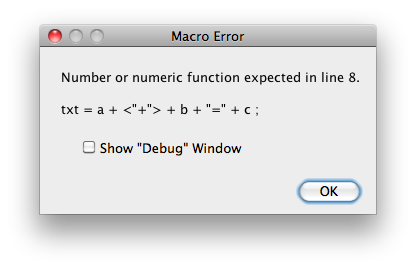
\includegraphics[scale=0.6]{fig/ErrorStringNumericFunction.png}
\caption{Error with Variable Assignment} \label{fig_ErrorVariable}
\end{center}
\end{figure}

This is because when ImageJ scans through the macro from top to bottom line by line, 
it reaches the txt substitution line and first sees the variable a and interprets that txt should be a numerical variable 
(or function), since a is a number. Then ImageJ goes on with the scanning and then sees "+" which is a character. 
ImageJ cannot interpret String variable within a numerical function. 

Instead, the programmer can tell ImageJ that 
\textit{txt} is a string function at the beginning of the function 
by putting a set of double quote at the beginning. 
ImageJ does handle numerical variables within string function, 
so the line works and prints out the result successfully.  

\begin{indentexercise}{2}
Modify the code 4, so that the calculation involves subtraction (-), multiplication (*) and division (/). 
\end{indentexercise}

\subsection{Parameter Input by User}
In many cases you may want to make a macro to ask the user to input some numerical values, 
file names. We learn how to do this here by first examining the following code. 
\lstinputlisting{code/code05.ijm}
Running this macro,  a dialogue window pops-up.

\begin{figure}[htbp]
\begin{center}
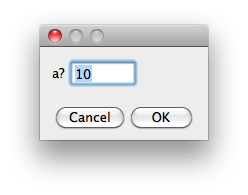
\includegraphics[scale=0.6]{fig/getNumberDialog.png}
\caption{getNumber Dialog} \label{fig_getNUmber}
\end{center}
\end{figure}

The command \textit{getNumber} consists of two parameters (programmers call such parameters "arguments").
\begin{indentCom}
\textbf{getNumber}(message string, default number)
\end{indentCom}
The first parameter is a string bounded with double quotes (see code 5, line 3 and 4). 
This string will appear in the dialogue window such as shown above. 
Default number will also appear in the dialogue window, 
and the user modifies this number. 
Then the number will be returned and then substituted to the variable a in the macro. 

To ask a string to users, following is an easy example. 
\lstinputlisting[morekeywords={*, getString}]{code/code06.ijm}

The command \textbf{getString} also has two arguments, and only the difference is that the user input will be treated as string parameter. \\

\begin{indentexercise}{1}
Run the code 6 and input 1 for a and 2 for b. What happened? Explain the reason. 
\end{indentexercise}

\subsection{Including ImageJ commands into a macro}
There are many functions in ImageJ. All these commands can be accessed from macro. 

We will make a macro that creates a new image, add noise,  blurs this image by Gaussian blur, 
and then thresholding the image. To know the commands we need there is a very convenient tool called 
"Command Recorder". 
Do \ijmenu{[PlugIns -> Macros -> Record\ldots]}. A window like below then opens. 

\begin{figure}[htbp]
\begin{center}
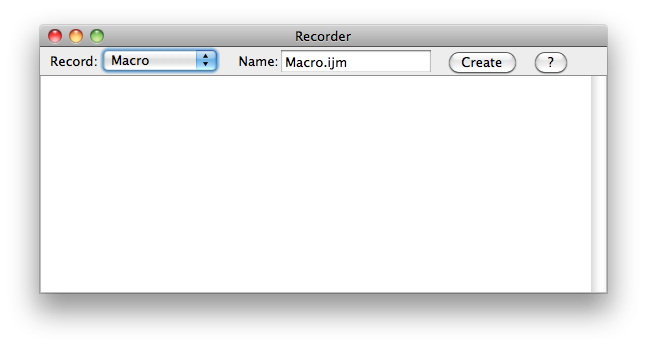
\includegraphics[scale=0.6]{fig/MacroRecorderBlank.png}
\caption{Macro Recorder} \label{fig_macroRecorderBlank}
\end{center}
\end{figure}

All the commands you will execute will be recorded in this window. 
So we first do the processing manually. 
Prepare a new image using [File -> New] command. 
Size of the image can be anything. 
Then do \ijmenu{[Process -> Noise -> Salt and Pepper]} (Fig. \ref{fig_SaltAndPepper}).

\begin{figure}[htbp]
\begin{center}
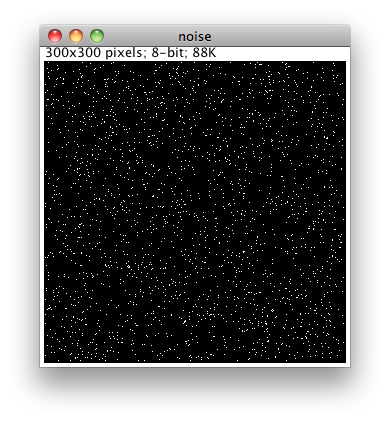
\includegraphics[scale=0.6]{fig/SaltandPepper300.png}
\caption{A demo image for Recording Macro} 
\label{fig_SaltAndPepper}
\end{center}
\end{figure}

\ijmenu{[Process -> Filters -> Gaussian Blur]} (use Sigma = 2.0).
then
\ijmenu{[Image -> Adjust -> Threshold\ldots]}. 
Toggle the slider to make signals red. Then click "Apply". Check "Dark Background" and OK. 

Now, check the Command Recorder window. 
It should now look like Fig. \ref{fig_macroRecorderFilled}. 
Lines appeared after your operations are corresponding commands.

\begin{figure}[htbp]
\begin{center}
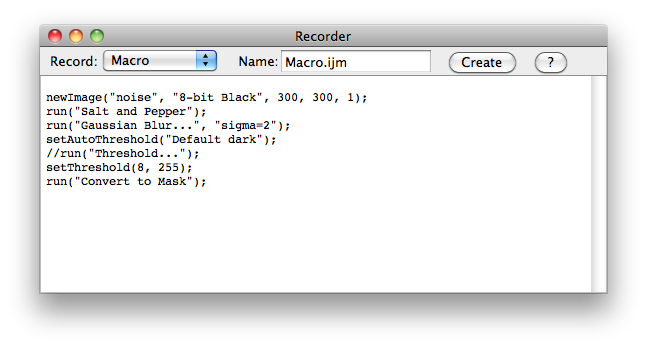
\includegraphics[scale=0.6]{fig/MacroRecorderFilled.png}
\caption{Macro Recorder after some lines Recorded} 
\label{fig_macroRecorderFilled}
\end{center}
\end{figure}

These lines appeared in the recorder can be used as it is. 
So you could copy and paste them to your macro. 
Prepare a macro like below, by copy and pasting the commands in the recorder. 
Delete the lines that is commented out 
(lines that begins with "//" are lines that are skipped by the macro interpreter).
\lstinputlisting{code/code07.ijm}

Try the macro! (I hope that you are amazed by now with the power of Macro Recorder!)\\
 
The second line in the above macro creates a new image. 
This command has many parameters (in coding jargon, we say "5 arguments"). 
To know what these parameters are, 
the quickest way is to read the Build-In Macro Function page in ImageJ web site  
(the reference is attached to this manual so take a look).  
In case of newImage command, the description looks like this. 

\begin{indentCom}
\textbf{newImage}(title, type, width, height, depth)\\
Opens a new image or stack using the name title. 
The string type should contain "8-bit", "16-bit", "32-bit" or "RGB". 
In addition, it can contain "white", "black" or "ramp" (the default is "white"). 
As an example, use "16-bit ramp" to create a 16-bit image containing a grayscale ramp. 
Width and height specify the width and height of the image in pixels. 
Depth specifies the number of stack slices.
\end{indentCom}
Using this information, you can modify the macro to change the size of the image. 
It is also possible to use variables as parameter. 
You could modify macro, so that the macro asks you width and height of the new image such as:
\lstinputlisting{code/code08.ijm}

\begin{indentexercise}{1}
Modify the code 8, so that user can input the desired Gaussian sigma.
\end{indentexercise}


\subsection{Batch Processing using "batch macro" function}
In above macro, list of commands were wrapped inside macro "title"\{ code \} 
so that the commands could be executed by single selection from menu. 
To apply such commands for many images in a single folder 
(say you have one-thousand images you want to contrast enhance and also to Gaussian-blur), 
there are two ways. One way is to further extend the macro by adding file-accessing command and 
looping the commands (you will learn this later). 
Another way is to do such "batch processing" by copy and pasting list of commands 
in previous section to batch-processing interface. 
This function could be called by \ijmenu{[Process -> Batch -> Macro]}

\begin{figure}[htbp]
\begin{center}
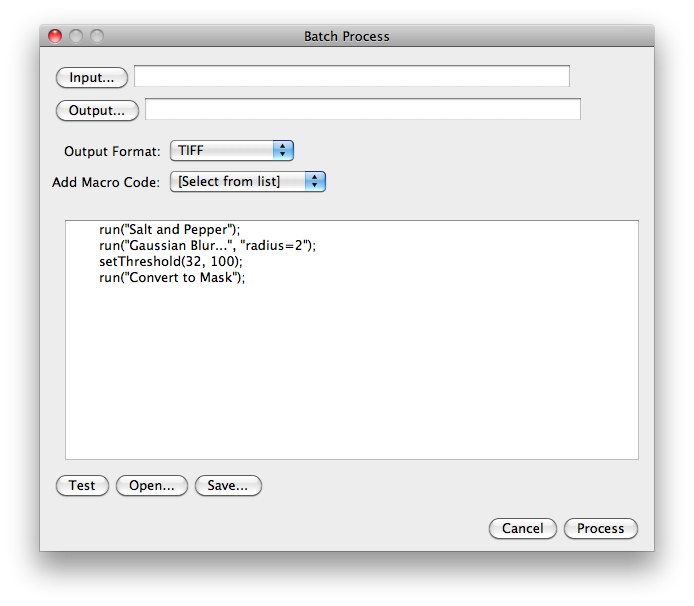
\includegraphics[scale=0.4]{fig/BatchProcessing.png}
\caption{Batch Processing Dialog} \label{fig_BatchProcessInterface}
\end{center}
\end{figure}

In "Input" field, select the folder where image files are stored. 
In output field, select a destination folder where processed images will be stored. 
You then copy and paste the list of commands in the code field such as 
shown in Fig. \ref{fig_BatchProcessInterface}. 
In the case shown in this figure, line 6 to 9 was copied and pasted. 
Clicking "Process" button will start the processing.
\newpage

\section{Conditions and Loops}
In many cases, we want to iterate certain processing many times ("Loops": see middle in the figure \ref{fig_scriptscheme}), or we want to limit some of the process in the program only for certain situations ("Conditions": see right of the figure \ref{fig_scriptscheme}). In this section we learn how to include these loops and conditional behaviors into macro. 

\begin{figure}[htbp]
\begin{center}
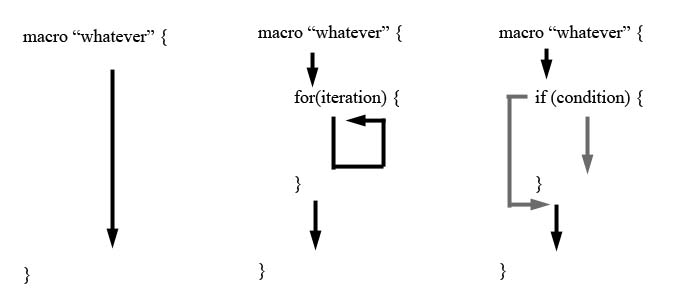
\includegraphics[scale=0.55]{fig/fig23_1_ScriptSchemes.png}
\caption{Schematic view of conditions and loops. Single line by line processing and macro with loops (middle) or with condition (right).} \label{fig_scriptscheme}
\end{center}
\end{figure}

\subsection{Loop: for-looping}
Here is a simple example macro using for-loop. Write the macro in your editor and run it. 
\lstinputlisting[morekeywords={*, for}]{code/code09.ijm}
The result should look like:

%whatever x 5 figure
\begin{figure}[htbp]
\begin{center}
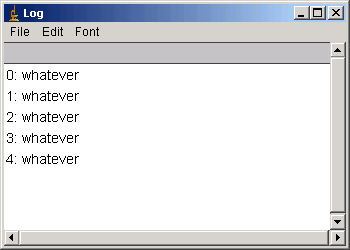
\includegraphics[scale=0.6]{fig/fig2311_whatever5.png}
\caption{Code 9 output in Log Window}
\label{fig_whateverOut}
\end{center}
\end{figure}

\begin{itemize}
\item Line 3 asks the user to input a string (we did this already). 
If user does not change the default text ("whatever") and click "OK", 
then the command interpreter proceeds to line 4.

\item Line 4 \ilcom{for(i=0; i<5; i+=1)} sets the number of looping. 
Three parameters are required for "for" loop. The first parameter defines the variable used for the counting loop and 
its initial value (\ilcom{i=0}). The second parameter sets the condition for exiting from the loop (\ilcom{i<5}). 
Third parameter sets the step size of i, meaning that how much value is added per loop (\ilcom{i +=1}, 
could also be subtraction, multiplication, division e.g. \ilcom{i-= 1}). 
\item After this \ilcom{for(\ldots;\ldots;\ldots)} command, there is a brace (\{) one at the end of line 4 (\{) and 
the second one in the line 6. These braces tell ImageJ to loop commands in between so command in line 5 will be iterated 
according to the parameters defined in the parenthesis of for. 
Between braces, you could add more lines of functions as much as you want.  
\end{itemize}
So when the command interpreter reaches line 4 and sees \ilcom{for(}, 
it starts looking inside the parenthesis and defines that the counting starts with 0 using a variable \ilcom{i}, 
and then line 5 is executed. The macro prints out "0 \ensuremath\colon whatever" 
using the content of \ilcom{i}, string \ilcom{\ensuremath\colon} and the string variable \ilcom{message\_txt}. 
Then in line 6, interpreter sees \ilcom{\}} and goes back to line 4 and adds 1 (because of \ilcom{i+=1}). 
i is still 1 so \ilcom{i<5} is true. The interpreter goes to line 5 and 
executes the command and prints out "1\ensuremath\colon whatever". 
Such looping will continue until i becomes 5, since when i becomes 5, 
\ilcom{i<5} is no longer true so interpreter goes out 
from the for-loop. \\

\begin{indentexercise}{1}
(1) Change the first parameter in \ilcom{for(i=0;i<5;i+=1)} so that the macro prints out only 1 line. 

(2) Change the second parameter in \ilcom{for(i=0;i<5;i+=1)} so that the macro prints out 10 lines. 

(3) Change the third parameter in \ilcom{for(i=0;i<5;i+=1)} so that the macro prints out 10 lines. 
\end{indentexercise}

\subsection{Stack Management by for-statement}
One of powerful application of for-loop in biological image processing is image stack management, 
such as measuring dynamics or multi-frame processing. 
Many ImageJ commands works with only single frame within a stack. 
Without macro programming, you need to execute the command while you flip the frame manually. 
Macro programming enables you to automate this process. 
Here is an example of measuring intensity change over time. 
\lstinputlisting[morekeywords={*, run, setSlice, nSlices}]{code/code10.ijm}
\begin{itemize}
\item Line 3: \ilcom{nSlices} is a command that returns number of slices in the active slice. 

\item Line 4: Sets measurement parameters. In this case "mean" intensity will be measured. 
You do not have to care for now about the "redirect" parameter. "decimal" This is the number of digits to 
the right of the decimal point in real numbers displayed in the results table. 

\item Line 5: clears the results table. 

\item Line 6 to 9 is the loop. Loop starts from count i=0, and ends at i=frame-1. Increment is 1.  

\item Line 7: calculates the current frame number. 

\item Line 8: \ilcom{setSlice} command set the frame according to the frame number calculated in line6. 

\item Line 9:  actual measurement is done. 
Result will be recorded in the memory and will be displayed in the Results table window. 
\end{itemize}

Open an example stack \textbf{1703-2(3s-20s).stk}
\footnote{Some of you may realize that you used this sequence 
in the Image Processing / Analysis Course for learning 
Time Series Analyzer Plugin. Now, you can program similar 
device in macro. Good thing about the custom program 
is that you will be able to modify the program further to add more functions.}. 
This is a short sequence of FRAP analysis, 
so edge of the one of the cells is bleached and then fluorescence recovers by time. 
Select FRAPped region by ROI tool (such as in the figure below). 
Execute the macro. Results will be printed in the Results window (see see the table in the figure left). 

%%%figure frap seq and quantification
%\begin{figure}[htbp]
% \begin{minipage}{0.5\hsize}
%  \begin{center}
%   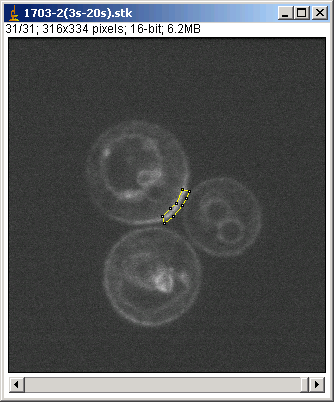
\includegraphics[height=50mm]{fig/fig2321a_frapimage.png}
%  \end{center}
%  \caption{Setting a Segmented ROI at the FRAPped area}
%  \label{fig:FRAProi}
% \end{minipage}
% \begin{minipage}{0.5\hsize}
% \begin{center}
%  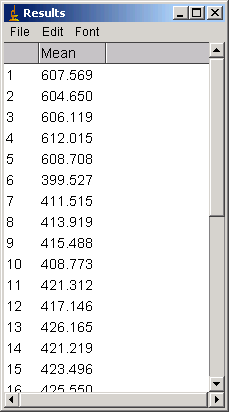
\includegraphics[height=50mm]{fig/fig2321b_frapResults.png}
% \end{center}
%  \caption{Results of Measuring Mean Intensity Dynamics}
%  \label{fig:MeanIntensityTimeCourse}
% \end{minipage}
%\end{figure}

%\begin{figure}[htbp]
% \begin{center}
%  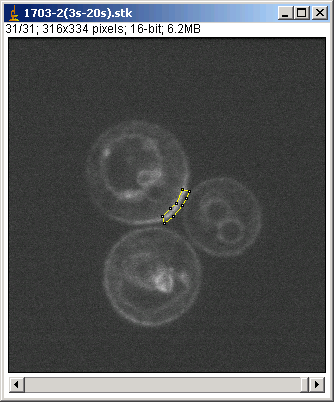
\includegraphics[height=50mm]{fig/fig2321a_frapimage.png}
%  \hspace{15mm}
% 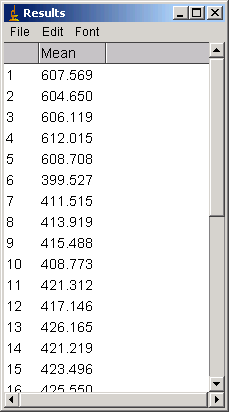
\includegraphics[height=50mm]{fig/fig2321b_frapResults.png}
% \caption{Left: Setting a Segmented ROI at the FRAPped area. Right: Results of Measuring Mean Intensity Dynamics.}
% \label{FRAPdynamics}
%\end{center}
%\end{figure}

\begin{figure}[htbp]
 \centering
% \subfloat[Setting a Segmented ROI at the FRAPped area.]{\label{fig:gull}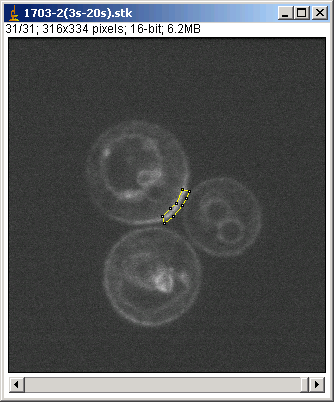
\includegraphics[width=0.3\textwidth]{fig/fig2321a_frapimage.png}}
 \subfloat[]{\label{fig:frapimage}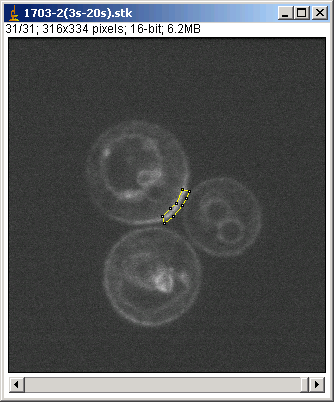
\includegraphics[height = 60mm]{fig/fig2321a_frapimage.png}}
 \subfloat[]{\label{fig:frapmeasured}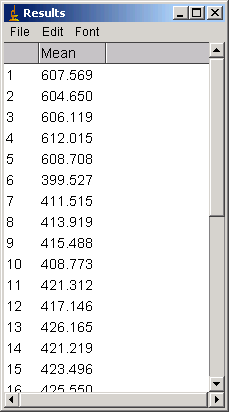
\includegraphics[height = 60mm]{fig/fig2321b_frapResults.png}}
 \caption{Measuring Stack Intensity Series. (a) Setting a Segmented ROI at the FRAPped area. (b) Results of Measuring Mean Intensity Dynamics.}
 \label{fig:frapresults}
\end{figure}


Measurement parameters can be added by modifying the line 4 in the code 10. "Set Measurement" could be added with more parameters to be measured, and decimals could be increased (highlighted in bold).
\begin{indentCom}
\textbf{run}("Set Measurements\ldots", "  mean min integrated redirect=None decimal=4")
\end{indentCom}

\begin{indentexercise}{1}
Modify code 10 to include more measurement parameters (whatever you like), and test the macro. Check the results. 
\end{indentexercise}

% figure
\begin{figure}[htbp]
\begin{center}
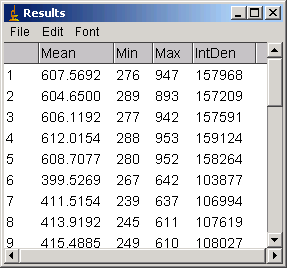
\includegraphics[scale=0.5]{fig/fig2322_moreResultsTable.png}
\caption{An example result after adding more measurement parameters.}
\label{fig_MoreMeasurementPara}
\end{center}
\end{figure} 

\subsection{Loop: while-looping}

Another way of letting part of macro to loop is \textbf{while}-statement. In this case, iteration is not defined strictly. Looping continues until certain condition is met. As soon as the condition is full-filled, macro interpreter goes out from the loop.

\subsubsection{Basics of while statement}
Here is a simple example macro using \ilcom{while}.
\lstinputlisting[morekeywords={*, while}]{code/code11.ijm}
This macro prints out characters 0 to 90 with a 10 increment. 

%figure
\begin{figure}[htbp]
\begin{center}
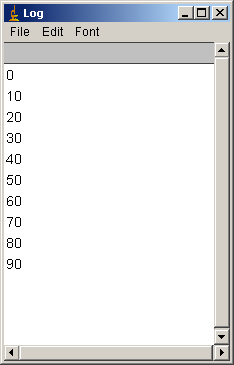
\includegraphics[scale=0.4]{fig/fig2331_Code11out.png}
\caption{Output of code 11}
\label{fig:code11 output}
\end{center}
\end{figure} 

\begin{itemize}
\item line 3: The macro interpreter first assigns 0 to the counter.
\item line 4: The interpreter evaluates if the counter value is less than or equal to 90. Since counter is initially 0\ldots 
\item line 5 Printing command is executed. 
\item line 6: counter is added with 10. 
\item line 7: the interpreter realizes the end of "while" boundary and goes back to line 4. Since counter= 10 <= 90, line 5 is again executed\ldots and so on. When counter becomes 100 in line 6 after several more loops, counter is no longer <=90. So the interpreter goes out from the loop, moves to line 8. Then the macro is terminated.
\end{itemize}

Line 5 could be written in the following way as well.
\begin{lstlisting}[numbers=none]
counter += 10;
\end{lstlisting}
This means that "counter" is added with 10. Similarly, subtracting 10 from counter is 
\begin{lstlisting}[numbers=none]
counter -= 10;
\end{lstlisting}
Multiplication is 
\begin{lstlisting}[numbers=none]
counter *= 10;
\end{lstlisting}
Division is
\begin{lstlisting}[numbers=none]
counter /= 10;
\end{lstlisting}
If the increment is 1 or -1, (counter +=1 or counter-=1), then one could also write them  as 
\begin{lstlisting}[numbers=none]
counter++;
 or 
counter--;
\end{lstlisting}
These two last commands are said to work faster than +=1 or -=1, but I myself do not see much difference. Computer is fast enough these days. 

\begin{indentexercise}{1}
(1) Try changing code 11 so that it uses "+=" sign.\\
(2) Change code 11 so that it uses "++" sign, and prints out integers from 0 to 9.\\
\end{indentexercise}
Evaluation of \ilcom{while} condition could also be at the end of loop. In this case, \ilcom{do} should be stated at the beginning of the loop. With do-while combination, the loop is always executed at least once, regardless of the condition defined by \ilcom{while} since macro interpreter reads lines from top to bottom. Try with the following exercise.

\begin{indentexercise}{2}
Change line 4 of code 11 to \ilcom{while (counter <0)} and check the effect (see below).
\end{indentexercise}

\lstinputlisting[morekeywords={*, while}]{code/code11_5.ijm}

Condition for the while-statement could be various. Here is a small list of comparison operators.

\begin{indentCom}
 \begin{tabular*}{0.5\textwidth}{ l r }
< & less than \\
<= & less than or equal\\ 
> & greater than\\ 
>= & greater than or equal to\\
== & equal\\
!= & not equal\\
 \end{tabular*}
\end{indentCom}

\begin{indentexercise}{3}
Modify code 11 so that the macro prints out numbers from 200 to 100, with an increment of -10. 
\end{indentexercise}

\subsection{Conditions: if-else statements}
\subsubsection{Introducing if-else}
A macro program could have different subroutines which are executed depending on the conditions. Here is an example of macro with conditions.  
\lstinputlisting[morekeywords={*, if}]{code/code12.ijm}
\begin{itemize}
\item Line 3 The macro asks user to input a number and the number is substituted to the variable input\_num.
\item Line 4 Content of input\_num is evaluated. If input\_num is equal to 5, line 5 is executed and prints out the message in the Log window. Otherwise macro interpreter jumps to line 7, and ends the operation.  By adding "else" which will be executed if input\_num is not 5, the macro prints out message in all cases (see code 12.5 for this if - else case). 
\end{itemize}

%figure
\begin{figure}[htbp]
\begin{center}
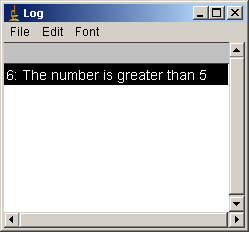
\includegraphics[scale=0.6]{fig/fig2341_code12out.png}
\caption{Output of code 12}
\label{fig:code12 output}
\end{center}
\end{figure} 

\lstinputlisting[morekeywords={*, if, else}]{code/code12_5.ijm}

We used double equal signs for comparison (e.g. "if (a==5)" ). Note that this functional role is different from assignments, or substitution (e.g. "a = b + c").

\subsubsection{Complex Conditions}
In many cases, you might need to evaluate the condition of multiple parameters at once. For such demands, several different comparisons can be combined by using following Boolean operators. 

\begin{indentCom}
 \begin{tabular*}{0.5\textwidth}{ l l }
\&\& & boolean AND\\
|| & boolean OR\\
\end{tabular*}
\end{indentCom}
Hers is an example.
\lstinputlisting[morekeywords={*, if, else}]{code/code12_75.ijm}
\begin{itemize}
\item Line 4 and 5 Ask user to input two parameters.
\item Line 6 is for setting a string variable, to abbreviate a long string assignment that appears four times in the macro.
\item Line 7 evaluates these input parameters by comparing each of them separately, but the decision is made by associating two decisions by "\&\&". 
\item Text after "//" is called comment. Text after this double slash will not be evaluated by the macro interpreter. Comments helps programmers later for remembering (or letting other programmer to understand) the purpose of the line. 
\item Line 10, != compares left and right sides of the operators and returns true if they are NOT equal.   
\end{itemize}
From line 10 to 17, there are several layers of conditions. Macro programmer should use tab-shifting for deeper condition layers as above for the visibility of code. Easy-to-understand code helps the programmer oneself to debug afterward, and also for other programmers who might reuse the code.
\subsubsection{Application of if-statement}
\label{sec:dotmove}
We make a macro that produces an animation of moving dot. User inputs the speed of the dot, and then the animation is generated. The dot moves horizontally and bounces back from the edge of the frame. “if�Eis used to switch the movement direction. 
\lstinputlisting[morekeywords={*, setForegroundColor, setBackgroundColor, if}]{code/code13.ijm}

\begin{itemize}
\item Lines 4 to 11: Set parameters for drawing a dot. It is also possible to directly use numerical values in the later lines, but for the sake of readability of the code, and also for possible later extension of the code, it is always better to use easy-to-understand variables and explicitly define them like in these lines. 
\end{itemize}
A short note on the x-y coordinate system in digital images: Since digital image is a matrix of numbers, each pixel position is represented as coordinates. The top left corner of image is the position (x, y) = (0, 0). X increases horizontally towards right side of the image. Y increases vertically towards the bottom of the image.  In line 9, y-position of the dot is defined to be placed in the middle of the vertical axis. 
\begin{itemize}
\item Lines 14, 15: These lines set the drawing and background color. Three parameters are for each RGB components. Here the image is in grayscale so all the RGB components are set to the same value. 0 is black, and int = 255 = white.
\item Line 14 asks the user to input the speed of the dot movement.
\item Lines 16, 17 prepares a new stack with parameters defined in lines 7, 8 and 9.
\item Lines 21 to 34 is the loop for drawing moving dot. Loop will be iterated from the starting frame until the last frame. Line 21 creates an oval ROI, which will be filled in line 22 with the foreground color that was already set in the line 14. \ilcom{makeOval} command is explained in the Built-on function page as follows.

\begin{indentCom}
\textbf{makeOval}(x, y, width, height)\\
Creates an elliptical selection, where (x,y) define the upper left corner of the bounding rectangle of the ellipse. 
\end{indentCom}
\item Line 27: Shifts the x position of the dot by ``speed'' distance. 
\item Line 28: if the position calculated in the line 27 exceeds the boundary, either left \ilcom{(x\_position < 0)} OR right \ilcom{(x\_position > (w-sizenum))}, then the direction of movement is switched by multiplying -1.
\end{itemize}
\begin{indentexercise}{1}
Modify code 13 that the dot moves up and down vertically. Change the stack width and height as well. 
\end{indentexercise}

\subsubsection{Application of "while" and "if" in image processing.}
Now, we try solving a problem with image thresholding by an application of 
\ilcom{while} loop in a macro. Open image \textbf{mt\_darkening.tif} in the sample image you downloaded. 
This is a stack, so you could slide the bar at the bottom of the window to see what is happening: 
the image gets darker and darker, as frame number increases. When you study fluorescence images, 
you will find such effect very often, because fluorescence bleaches due to the irradiated excitation light 
for the acquisition. 
When you want to segment this structure (a microtubule), you might use image-thresholding as follows. 

%figure
\begin{figure}[htbp]
\begin{center}
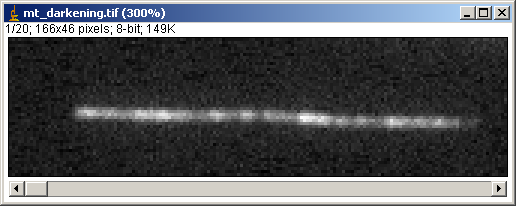
\includegraphics[scale=0.6]{fig/fig23441_mtStack.png}
\caption{A stack with darkening microtubule}
\label{fig:MTstack}
\end{center}
\end{figure} 

Go back to the first frame and do \ijmenu{[Image -> Adjust -> Thresholding\ldots]}. The image is then automatically adjusted with threshold level. and it seems Ok that the structure is well segmented. But the problem appears as you slid the bar at the bottom. Since image is darkening, area where highlighted decreases. 

%figure
\begin{figure}[htbp]
 \centering
 \subfloat[]{\label{fig:frame1Th}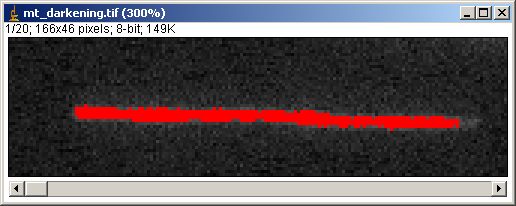
\includegraphics[height = 20mm]{fig/fig23442a_frame1threshold.png}}
 \subfloat[]{\label{fig:framelastTh}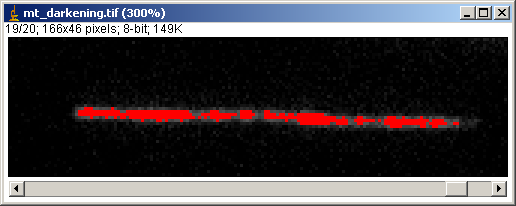
\includegraphics[height = 20mm]{fig/fig23442b_frameLastthreshold.png}}
 \caption{Adjusted with threshold level first frame (a) and the last frame (b)}
 \label{fig:degradingThreshold}
\end{figure}

This is because the threshold minimum and the maximum is kept constant while the intensity of the image is decreasing. To segment the structure while the image darkening is occurring, we must adjust the threshold intensity range as the frame progresses. 
 
The macro below finds the minimum value for the thresholding, that the highlighted area in each frame in a stack is approximately similar to the first frame. \ilcom{while} is used to loop the adjustment until the highlighted area is constant.  Then the threshold is applied to the image to convert the stack to a binary stack. 

\lstinputlisting[morekeywords={*, getThreshold, getSliceNumber, getImageID, getResult, while, setThreshold}]{code/code14.ijm}

%figure
\begin{figure}[htbp]
 \centering
 \subfloat[]{\label{fig:binMTorg}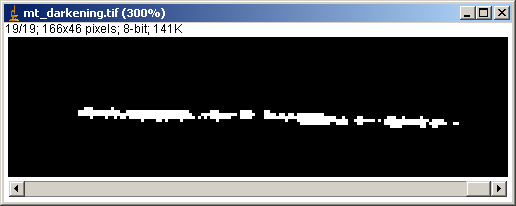
\includegraphics[height = 20mm]{fig/fig23443a_framelastbinOrg.png}}
 \subfloat[]{\label{fig:binMTproc}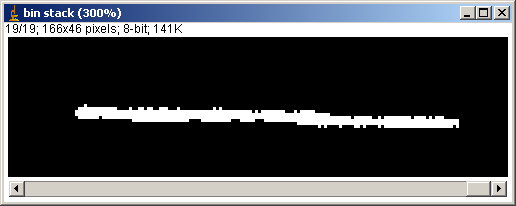
\includegraphics[height = 20mm]{fig/fig23443b_framelastbinProc.png}}
 \caption{Binarized last frame without threshold adjustment (a) and with adjustment using macro (b).}
 \label{fig:ThresholdAdjustResults}
\end{figure}

\begin{itemize}
\item Lines 3 to 5 Check if the active window is a stack. If \ilcom{nSlices==1} (meaning that the image is not a stack), macro is terminated. 

\item Lines 6 to 9: Get the threshold parameter from image and check if the image is adjusted with threshold level. If not, both upper and lower values are -1. In this case, macro is terminated. 

\item Lines 10 to 14: Get stack information. \ilcom{getSliceNumber()} returns the current frame in the stack. Adjusted with threshold level area in this frame (first frame) will be used as the reference area. \ilcom{getImageID()} returns a number that specifically identifies the active window. This ImageID will be used later,by \ilcom{selectImageID(ImageID)} to re-activate the window. 
%\end{itemize}

\begin{indentCom}
\textbf{getImageID()}\\
Returns the unique ID (a negative number) of the active image. Use the selectImage(id), isOpen(id) and isActive(id) functions to activate an image or to determine if it is open or active. 
\end{indentCom}
%\begin{itemize}
\item Line 16: clears the results table without saving. 

\item Line 17: sets the measurement parameter Area, and limits the measurement to the adjusted with threshold level region. 

\item Line 18: Do the measurements. Result is recorded in the first row of the Results table.

\item Line 19: The measured area is stored in the variable ref\_area. 

\item Line 20: temp\_area will be used later in the while loop. 

\item Line 21: the variable ilcom{tol} is a tolerance ratio of error against the reference area. So the adjusted with threshold level area in each frame should be between 97 and 103\% of the reference area. 

\item Line 22: Create a destination stack, where adjusted with threshold level images will be pasted. 

\item Line 23: get the Image ID of newly created image. 

\item Line 25: Loop for the frames starts. 

\item Lines 26, 7: Select the original stack and sets the frame number according to the loop number. \ilcom{selectImageID} works with \ilcom{getImageID} command in line 14. 


\begin{indentCom}
\textbf{selectImage(id)}\\
Activates the image with the specified ID (a negative number). If id is greater than zero, activates the idth image listed in the Window menu. With ImageJ 1.33n and later, id can be an image title (a string).
\end{indentCom}

\item Line 28: Copy the full frame.

\item Lines 29, 30: creates a temporally single frame image and the image copied in line 28 is pasted. 

\item Lines 31 to 37: While loop. temp\_area is evaluated if the area is outside 97 and 103\% of the reference area. If true, then loop continues. Initial temp\_area value is 0 so the loop is at least one time. Set Threshold with lower and upper (line 32). Measure the adjusted with threshold level area, and then lower is incremented -1. The area is evaluated, and if it does not meet the criteria set in line 31, then the loop continues with wider threshold range. 

\item Lines 38 to 40: The adjusted with threshold level image will be converted to black \& white image and then copied. The single frame temporary image is closed.

\item Line 41, 42: destination stack is activated and the same frame as the source stack is set. 

\item Line 43: Binarized image in the clipboard is pasted into the destination stack.

\item Line 44: returns to Line 25 until all stack frames are processed.

\item Line 45: Terminates the macro. 
\end{itemize}

\newpage

\section{Advanced Macro Programming}
This section could be a bit boring for you in terms of biology, but try to be patient. 
All these knowledge are required for advanced programming. 
Ability to do complex image processing using macro widens your view on planning experiments also.

\subsection{User-defined Functions}
As the code you write becomes longer, 
you will start to realize that similar processing or 
calculation appears several times in a macro or through macro sets. 
To simplify this redundancy, one could write a 
separate \ilcom{function} that works as a module for macros. 
For example, if you have a simple code like:
\lstinputlisting[morekeywords={*,}]{code/code15.ijm}
It should be easy for you to expect that this macro will print out "3" in the Log window. 
From this macro, we could extract part of it and and make a separate function. 
\lstinputlisting[morekeywords={*,}]{code/code15_1.ijm}
This is not a macro, but is a program that works as a unit. 
Functions can be embedded in macro. \ilcom{ReturnAdd }(code 15.1) is the name of the function, 
and the following (n, m) are the variables that will be used in the function. Within the function, 
n and m will be added and the result of which is substituted in to a new variable p. 
\ilcom{return p} in line 4 will return a value as an output of the function. 
In a sense, this is a custom made Macro function. Using this function, code 15 can be rewritten as
\lstinputlisting[morekeywords={*,}]{code/code15_2.ijm}
or more simply, by nesting the custom made function inside ImageJ native function \ilcom{print()},
\lstinputlisting[morekeywords={*,}]{code/code15_3.ijm}
Macro interpreter reads the macro line by line. When the interpreter sees \ilcom{ReturnAdd(a, b)}, 
the interpreter first tries to find the function within the ImageJ Build-in function. 
If its not there, the interpreter looks for the function within the same macro file\ldots 
(user-defined function (e.g. \ilcom{ReturnAdd(a, b)} must be written in the same macro file. 
Here is how it looks like: a macro that uses a function. 
%figure
\begin{figure}[htbp]
\begin{center}
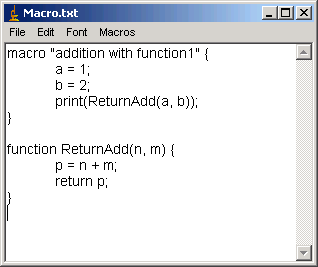
\includegraphics[scale=0.6]{fig/fig2411_usingFunction.png}
\caption{A macro file with function}
\label{fig:MacroWithFunction}
\end{center}
\end{figure} 

In this simple case, 
you might not feel the convenience of the User-defined function, 
but you will start to feel its power as you start writing longer codes. 
Advantages of using \ilcom{function} are
\begin{enumerate} 
\item Once written in a macro file, it could be used as a single line function 
as many times as you want in the macro file. This also means that if there is a bug, 
fixing the function solves the problem in all places where the function is used.
\item Long codes could be simplified to an explicit outline of events. Such as:
\begin{lstlisting}[numbers=none]
macro "whatever" {
		function1;
		function2;
		function3;
}
\end{lstlisting}
\end{enumerate}

Let's go back to the code 14, the automatic threshold adjusting macro. 

At the beginning of the code, we check if the active image if it is a stack. 
There is another check after that, to see if the image is adjusted with threshold level.

\lstinputlisting[linerange={1-10}]{code/code14.ijm}

We can make a function for checking stack (line 3 to 5) and another function that checks 
if the stack is adjusted with threshold level (from line 6 to 9) as below.

\lstinputlisting{code/code16_17functions.ijm}

Then the initial part of code 14 (line 3 to 9) can now be replaced with 
these two functions\footnote{For a complete coding of 14.1, 
getThreshold(lower, upper) should appear again in line 8 to get lower and upper threshold value 
of the reference image.}. 

\lstinputlisting[linerange={1-5}]{code/code14_1.ijm}

\begin{indentexercise}{1}
The following macro asks the user to input x and y coordinates of two points, 
calculate the distance between those points and prints out the distance. 
Modify the code so that the distance calculation is done in a separate function. 

\lstinputlisting{code/code18.ijm}

Note that function \ilcom{pow()} in the code is defined as
\begin{indentCom}
\textbf{pow}(base, exponent)\\
Returns the value of base raised to the power of exponent. 
\end{indentCom}
For example, \ilcom{pow(4, 2)} returns 16.
\end{indentexercise}

\subsection{Multi-parameter dialogue}
In code 18 we examined above, 
user-interface is very poor since before calculation the user must input\ldots 
click\ldots input\ldots click\ldots for total of four times. 
To ease this exhausting series of input process, 
you could create a dialog box that asks the user to input several parameters at once. 
We use \ilcom{Dialog} functions. 

\lstinputlisting[morekeywords={*, Dialog, create, addMessage, addNumber, addCheckbox, show, getNumber, getCheckbox}]{code/code18_5.ijm}

%figure
\begin{figure}[htbp]
\begin{center}
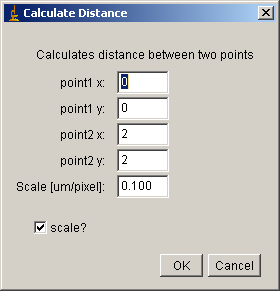
\includegraphics[scale=0.6]{fig/fig2421_GenDialog.png}
\caption{Custom Parameter Input Dialog}
\label{figGenericDialog}
\end{center}
\end{figure} 

Line 2 to 9 creates a dialog box that has multiple input boxes that looks like Fig. \ref{figGenericDialog}. 

\begin{itemize}
\item Line 3 defines the title of the dialog window. 


\item Line 4 texts will be shown within the window. 

\item Line 5 to 11 defines the parameter input fields. Fields appear in the dialog box in the order of lines with Dialog.addNumber command in the macro. When you press OK button in the dialog box, parameter will be stored in the same order. 

\item Line 15 to 19 These values then are assigned to each variable by Dialog.getNumber(). 

\item Line 20 Checkbox is independent from these number fields and the value is returned by \ilcom{Dialog.getCheckbox()}. When you check the check box, the return value is 1. If not, the return value is 0. We use this Boolean value (true or false)  to decide if the scale will be multiplied to the distance [pixel] in Line 24.

\item Line 24 This if-statement does not have braces. Such simplification is possible if there is one line when "if" is true.  
\end{itemize}

You may also realize that the if statement in line 24 (and also in Line 28) does not have comparison like == or <  or so on. This is because \ilcom{switchscale} takes only 0 or 1 (\textbf{boolean}), which are interpreted as true ( \ilcom{switchscale} = 1) or false ( \ilcom{switchscale} = 0). So even without comparison, \ilcom{switchscale} is already a decision.  

\begin{indentexercise}{1}
Modify Code 5 so that two parameters are asked in a single dialog box. 
\end{indentexercise}

\subsection{Global Variables}

"Global variables" are variables that are defined outside macro or function within the same macro file. So what is good about Global variables? For instance in Code 18.5, we had a variable called \ilcom{scale}. \ilcom{scale} had to be typed every time when you execute the macro. One way to avoid such tedious interaction with the program is forget about the line 10 and 19, where the user input is asked for the \ilcom{scale}, and instead place something like
\begin{lstlisting}[numbers=none]
scale = 0.1
\end{lstlisting}
somewhere at the beginning of the macro. This works OK, but the problem appears 
when there are many macros in the file, since it will be a loads of work to 
find the variable \ilcom{scale} in the file and change the value. 
It could also be that the name of variable is not \ilcom{scale} and something like \ilcom{pixelsize}, 
which then you have to check what this variable is doing. Furthermore, 
it becomes redundant if you need to calculate the scale in every macro. 
For this reason, you could define the scale only once in the macro file such that:

\lstinputlisting[linerange={1-20}, morekeywords={*, Gscale}]{code/code18_75.ijm}

\ilcom{var} is a statement that tells macro interpreter to treat the variable as a global variable. 
It should be always outside the scope (braces) of macro or function. 
I replaced the default value in the scale input field of the \ilcom{dialog.addnumber()} at line 11 
to \ilcom{Gscale}, so that the initial value defined in line 2 appears in the dialog box. 
The value in the field could be modified by the user, 
but this does not affect the \ilcom{Gscale} value defined in Line 2. 
This is because the flow of information is:

\ilcom{Gscale} \\
\tab > default value for the \ilcom{Dialog.addNumber} field 5 \\
\tab\tab > user changes the value  \\
\tab\tab\tab > stored in the \ilcom{Dialog.addNumber} field 5\\
\tab\tab\tab\tab > scale = \ilcom{Dialog.getNumber} (field 5)\\

So \ilcom{Gscale} is referenced, but not modified. 
If you want to change the Global value from inside the macro, you must redefine by such as
\begin{lstlisting}[numbers=none]
Gscale = scale;
\end{lstlisting}
In the macro set below, we test the use of global variable (+ function!). 
The macro is for the conversion of pixel length into micrometer. 
The second macro changes the scale value. 
I usually put G for all global variable. This is not necessary, 
but in a file with many macros this is convenient.
\lstinputlisting[morekeywords={*, G_scale}]{code/code19_globalVariable.ijm}
\begin{indentexercise}{1}
Add another global variable G\_scale\_z ( [\ensuremath{\mu}m]) for storing spacing in z-axis. 
Change the first macro, that it calculates the size of Voxel in um3. 
Then add another macro for changing the scale in Z axis. 
\end{indentexercise}

\subsection{String Arrays}
Array is a powerful tool. before going into how to use it, here is an easy explanation. 
Imagine that an array is a stack of boxes. Boxes could contain either numbers or strings. 
For instance, if you have a following list of strings:

\textit{Heidelberg, Hamburg, Hixton, Grenoble, Monterotondo}

An array "EMBL" could be prepared that the array element will contain these 5 strings. 

 %figure
\begin{figure}[htbp]
\begin{center}
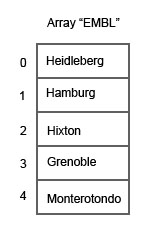
\includegraphics[scale=0.6]{fig/fig2441_arrayScheme.jpg}
\caption{EMBL array}
\label{figEMBLarray}
\end{center}
\end{figure} 
 
Then when you want to retrieve some name, you refer to the address within the array. 
So EMBL[0] will be Heidelberg, EMBL[4] will be Monterotondo, and so on. 
In such a way, files names contained in a folder could be listed and stored, 
or x-y coordinates of free-hand ROI could be stored for further use. 

Here is a macro using the EMBL array example. 

\lstinputlisting[morekeywords={*, newArray}]{code/code20.ijm}

\begin{itemize}
\item Line 2 uses a command that creates a new array (\ilcom{newArray()}), defined by a parameter for number of array elements (in the example case its 5) and its name \ilcom{EMBL}. 
\item From line 3 to 7, each array from position 0 to 4 will be filled with names (Array starts with 0th element). 
\item Line 8 asks the user to input the address (position) within the array. Then this input address is examined if the address exists within the \ilcom{EMBL} array in line 9. \ilcom{EMBL.length} returns the number of "boxes" within the array. If this is satisfied, then line 10 prints out the string in that address.
\end{itemize}

\subsection{Numerical Array}

Array could also contain numerical values, and this way of usage is more common when you do image analysis. Here is a simple example of numerical array that prints out intensity profile along selected line ROI. 

\lstinputlisting[morekeywords={*, newArray, selectionType, getProfile, setResult, updateResults}]{code/code20_5.ijm}

\begin{itemize}
\item Line 3: Check if the selection type is a straight line ROI. If not, macro terminates leaving a message. 

\begin{indentCom}
\textbf{selectionType}()\\ 
Returns the selection type, where 0=rectangle, 1=oval, 2=polygon, 3=freehand, 4=traced, 5=straight line, 6=segmented line, 7=freehand line, 8=angle, 9=composite and 10=point. Returns -1 if there is no selection.
\end{indentCom}

\item Line 4: Empty array \ilcom{tempProfile} is loaded with the intensity profile along the line ROI by \ilcom{getProfile}().
\item
\begin{indentCom}
\textbf{getProfile}()\\
Runs Analyze/Plot Profile (without displaying the plot) and returns the intensity values as an array.
\end{indentCom}

\item Line 5: Passing the array \ilcom{tempProfile} to function "output\_results", which prints the content of array in Results window. 

\item Line 7 to 14: A function for outputting the profile array in the result table. It takes an argument \ilcom{rA}, which is supposed to be an array. 
\item Line 8: Clears the result table. 
\item Line 9 to 12: for-loop to go through the array and to print out each element. 
\item Line 10: Sets the pixel position along the segment in the column labeled "n". 
\item Line 11: Sets the content of the array (pixel intensity) in the column labeled "intensity".

\begin{indentCom}
\textbf{setResult}("Column", row, value)
Adds an entry to the ImageJ results table or modifies an existing entry. The first argument specifies a column in the table. If the specified column does not exist, it is added. The second argument specifies the row, where 0<=row<=nResults. (nResults is a predefined variable.) A row is added to the table if row=nResults. The third argument is the value to be added or modified. 
\end{indentCom}
\item Line 13: Updates the result table, so that above changes are actually reflected in the Result window. 

\begin{indentCom}
\textbf{updateResults}()
Call this function to update the "Results" window after the results table has been modified by calls to the setResult() function. 
\end{indentCom}
\end{itemize}

\begin{indentexercise}{1}
Modify code 20.5 that the macro calculates the sum of all intensity.\\
\begin{enumerate}
\item You do not need the function anymore. 
\item for-loop should be used.
\item Hint: use \ilcom{tempProfile.length}
\end{enumerate}
\end{indentexercise}

\subsection{Application of Array in Image Analysis}

Array is used in many built-in macro functions, especially for storing array of numerical values. Here is a list of functions which use array. 

\begin{indentCom}
\texttt{
\item Dialog.addChoice("Label", items) 
\item Dialog.addChoice("Label", items, default)
\item Fit.doFit(equation, xpoints, ypoints)
\item Fit.doFit(equation, xpoints, ypoints, initialGuesses)
\item getFileList(directory)
\item getHistogram(values, counts, nBins[, histMin, histMax])
\item getList("window.titles")
\item getList("java.properties")
\item getLut(reds, greens, blues)
\item getProfile()
\item getRawStatistics(nPixels, mean, min, max, std, histogram)
\item getSelectionCoordinates(xCoordinates, yCoordinates)
\item getStatistics(area, mean, min, max, std, histogram)
\item makeSelection(type, xcoord, ycoord)
\item newArray(size)
\item newMenu(macroName, stringArray)
\item Plot.create("Title", "X-axis Label", "Y-axis Label", xValues, yValues)
\item Plot.add("circles", xValues, yValues)
\item Plot.getValues(xpoints, ypoints)
\item setLut(reds, greens, blues)
\item split(string, delimiters) 
}
\end{indentCom}

To learn the actual use of Array in Image analysis, we use some of these functions and 
create a macro that reads and shows the line-profile from segmented line ROI. 
Similar function is already available ([Analyze > Plot Profilw]), 
but original function reads only single-pixel width profile from segmented line ROI. 
We extend this native function to enable sampling segmented line ROI with flexible width.

In the code below, there is only one macro. Three functions are added at the bottom. 
Two are for the plotting of the profile in a graph and the last one is for outputting 
the results in the result table. Strategy of this macro is to use straight line selection 
for each segment (custom thickness is available with straight line ROI). 

Since width of the profile could be set various, each segment is measured individually 
and then profiles are assembled afterwards. 

%\lstinputlisting[morekeywords={*, newArray, selectionType, getProfile, setResult, updateResults}]{code/code20_75.ijm}
\lstinputlisting[morekeywords={*, getSelectionCoordinates, makeLine, Plot, create, setLimits, setColor, add, show}]{code/code20_75.ijm}

\begin{itemize}
\item Lines 2, 3: global variables for setting the plot range (minimum and the maximum value of the y-axis) in the profile plot. Function from line 40 to 47 evaluates the measured profile and updates these values. 

\item Lines 5 - 36: Main part, macro for the segmented line ROI measurement.  

\item Line 6: Check if the selection type is a segmented line ROI. If not, macro terminates leaving a message. 

\item Line 7: This command reads the x and y coordinates of the segmented line into two arrays\ilcom{xCA} and \ilcom{yCA}.

\begin{indentCom}
\textbf{getSelectionCoordinates(xCoordinates, yCoordinates)}\\
Returns two arrays containing the X and Y coordinates of the points that define the current selection. 
\end{indentCom}

\item Line 8 - 10: asks the user to input width of the segmented ROI. The ROI line width is set to that value. 

\item Line 11 - 16: Measures the total length of the segmented profile, by actually setting straight line ROIs to each segment by \ilcom{makeLine} command, and get its intensity profile by \ilcom{getProfile()} command.  

\begin{indentCom}
\textbf{makeLine(x1, y1, x2, y2)}\\
Creates a new straight line selection. The origin (0,0) is assumed to be the upper left corner of the image. Coordinates are in pixels. With ImageJ 1.35b and letter, you can create segmented line selections by specifying more than two coordinate, for example makeLine(25,34,44,19,69,30,71,56).
\end{indentCom}

\item Profile data is assigned to a new array called tempProfile but the profile data is not used in this loop. Only the length of the array (\ilcom{tempProfile.length}) is used and added up to \ilcom{totalprofilelength} the measurement is done for each ROI segment. Line 17 prints out the result of these array length measurements in the Log window. 

\item Line 21: using the measured value \ilcom{totalprofilelength}, a new array \ilcom{totalprofile} is created. This new array stores the total profile. 

\item Line 22 - 33: Profile measurement using straight line selection in each segment. This time, profile data in \ilcom{tempProfile} array is transferred to \ilcom{totalprofile} array starting at the position \ilcom{segment\_starts} value. 

\item Line 34: call graph plotting function (Line 40 - 47) using \ilcom{totalprofile} array.

\item Line 35: call function to printout the profile array in the results window (Lines 60 - 67). 

\item Line 40 - 47: Function for plotting the intensity profile.
\item Line 41: Calls another function to determine the minimum and the maximum intensity of the profile (lines 50 - 56). 
\item Line 42: Creates the window and axes of the plot. 
\item Line 43: Set the range for x and y axis using the global variables \ilcom{PlotRange\_y\_min}  and \ilcom{PlotRange\_y\_max}. 5\% of offset is added to both values, to make spaces below and above. 
\item Line 44: Sets the color of the plot. 
\item Line 45: Plot the profile. 
\item Line 46: Show the plot on the screen (lot is hidden until this show() command).

\item Line: 50 - 57: Function for adjusting the y-axis range of profile plotting. 
\item Line 51 - 56: for-loop to scan through the array \ilcom{referenceA}. 
\item Line 52, 53: if a value in the array is larger than the maximum value stored in the global variable \ilcom{PlotRange\_y\_max}, then replace the value with the array value. 
\item Line 54, 55: if a value in the array is smaller than the minimum value stored in the global variable \ilcom{PlotRange\_y\_min}, then replace the value with that array value. 

\item Line 60 - 67: Function for outputting the profile array in the result table.  
This function is exactly the same function you studied in the previous chapter (code 20.5).

\end{itemize}

Length of array must be defined when the array is created and cannot be changed afterward. 
For this reason, this macro needs to first loops through segments to count the number of points (line 11 -16) to create an array for storing the full profile of the segemented ROI (line 21). Actual measurement of intensity profile is done in the second loop (line 22-33).

Such restriction on array usage (fixed array length) does not exist with other scripting languages 
such as Javascript or Jython, since array in these languages could be added with new elements after 
creating it. 

\newpage

\section{File I/O}

Analysis of images requires both input and out put: input is to load images, 
and output is  to save either processed images or numerical data. 
If number of image files or quantity data is manageable by manual loading and saving, 
we do not have to automate. But in some cases you need to process a huge number of files. 
This often happens especially after you establish a protocol and you want to get 
statistically sufficient amount of data. Then you need to automate file input and output using macro. 
Once you learn how to write File I/O program, you can process as much files as you want, 
as long as your memory space allows.

\subsection{Saving the Measurement Results Automatically}

When you have a time series sequence and you want to measure multiple signals with 
multiple parameters in each frame, measurement results in each frame needs to be somehow saved. 
Here, we learn how to export measurement results in your hard disk automatically using macro. 

Open the sample image \ilcom{Nucseq001.tif}. Cell nucleus shows that they divide and 
increase their number over time. We want to count the number of nucleus in each frame to know 
the dynamics of increase. 
At the same time, we may also want to see changes in the signal intensity and shape. 
For this measurement Particle Analysis function works best. Do the following:

\begin{enumerate}
\small{
\item \ijmenu{[Image -> Adjust -> Threshold]}. 
Threshold the image and check the threshold lower and upper value that segments the nucleus optimally. 
\item Set the measurement parameters. \ijmenu{[Analysis -> set measurements\ldots]}
\begin{enumerate}
\item Check Area, Mean intensity, centroid, Circularity and Slice number. 
\item Check "limit to threshold"
\item Digits after decimal point: 2
\end{enumerate}
\item \ijmenu{[Analyze -> Analyze Particles\ldots]}
\begin{enumerate}
\item Size: 10 - Infinity
\item Circularity = 0.5 - 1.0
\item Show: Outline
\item Check Display Results
\item Check Exclude on Edges
\item Check Clear Results
\end{enumerate}
\item Then click "OK". 
}
\end{enumerate}
After these steps, you will find outline image showing detected cells and a result table. 

%double figure
\begin{figure}[htbp]
 \centering
 \subfloat[]{\label{fig:thresholdCells}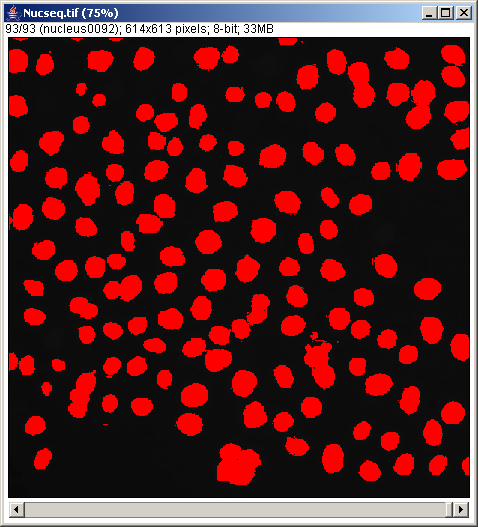
\includegraphics[height = 60mm]{fig/fig2511a_CellsThreshold.png}}
 \subfloat[]{\label{fig:ParticleAnalysisDialog}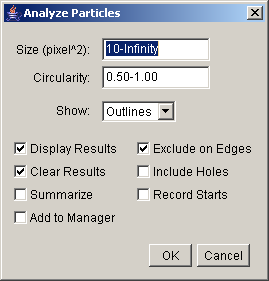
\includegraphics[height = 60mm]{fig/fig2511b_AnalyzeParticleDialog.png}}
 \caption{ (a) Thresholded cell image and (b) Particle Analysis parameter input dialog.}
 \label{fig:ParticleAnalysis}
\end{figure}

%double figure
\begin{figure}[htbp]
 \centering
 \subfloat[]{\label{fig:OutlinedCells}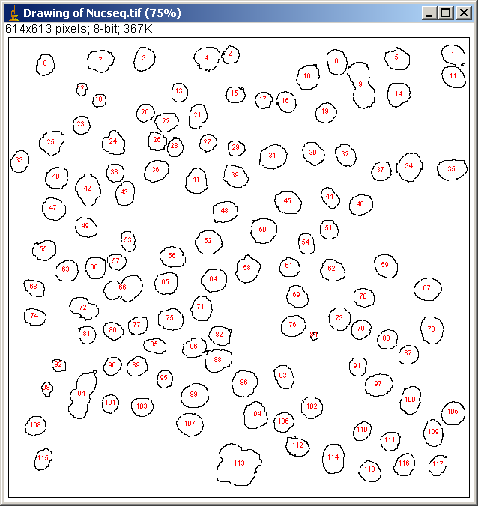
\includegraphics[height = 50mm]{fig/fig2511c_CellOutlines.png}}
 \subfloat[]{\label{fig:ParticleAnalysisResults}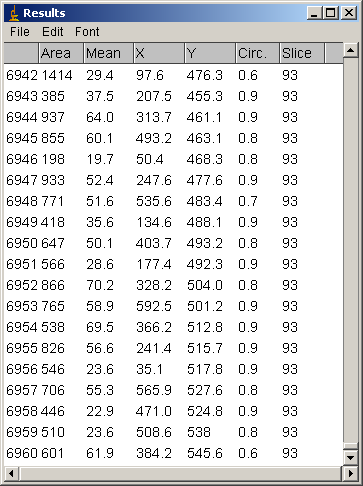
\includegraphics[height = 50mm]{fig/fig2511d_ParticleAnalysisResults.png}}
 \caption{ After particle analysis is done, (a) outlined cell image and (b) results table listing measurement results.}
 \label{fig:ParticleAnalysisResults}
\end{figure}

Using macro recorder, its easy to write a macro set as following. 

\lstinputlisting[morekeywords={*, }]{code/code21.ijm}

Two macros and a global variable consists this macro set. 
Global variable is a string variable that stores the path to the location where file will be saved. 
(note: path is differently written in MacOS. It uses slash instead of back-slash). 
The first macro \ilcom{Set Directory to save Results} is for setting the path to the folder 
(or directory) where the file will be saved. 
We use a command \ilcom{getDirectory(title)} to get user choice of a destination folder. 

\begin{indentCom}
\textbf{getDirectory(title)}\\
Returns the path to a specified directory. If title is "startup", returns the path to the directory 
that ImageJ was launched from (usually the ImageJ directory). If it is "plugins" or 
"macros", returns the path to the plugins or macros folder. If it is "image", 
returns the path to the directory that the active image was loaded from. 
If it is "home", returns the path to users home directory. 
If it is "temp", returns the path to the /tmp directory. 
Otherwise, displays a dialog (with title as the title), 
and returns the path to the directory selected by the user. 
Note that the path returned by getDirectory() ends with a file separator, 
either "\" (Windows) or "/". Returns an empty string if the specified directory is not found or 
aborts the macro if the user cancels the dialog box.
\end{indentCom}

When you run this first macro, global string variable \ilcom{G\_Ddir} 
will be set to a folder where user will select, and line 6 prints out the path to 
a folder (or directory). It might be convenient for you to change the default directory path 
in the code above (line 2), by copying the results in the log window and pasting it in the macro. 

The measurement macro starts from the Line 9. 
\begin{itemize}
\item Line 10 to 13: Checks if the image is thresholded. 
\item Line 14: Sets the threshold level. 
\item Line 15: Gets the title of the image window for later use. We use this for 
generating name of the results file.
\item Line 16: to 17: Sets the measurement parameter and does the actual 
particle analysis. Commands are direct copies from the recorder. 
\end{itemize}
After the analysis, we want to save the results. 
\begin{itemize}
\item Line 18: Generates the file name using the image file name stored in the line 15 by concatenating concatenate image title with \ilcom{\_measure.xls}. 
\item Line 19: The full path file name is constructed by adding the result filename generated in line 18 with path stored in the global variable. 
\item Line 20: Saving the result table as an excel-readable file uses a new command \ilcom{saveAs}:
\begin{indentCom}
\textbf{saveAs(format, path)}
Saves the active image, lookup table, selection, measurement results, selection XY coordinates or text window to the specified file path. The format argument must be "tiff", "jpeg", "gif", "zip", "raw", "avi", "bmp", "fits", "png", "pgm", "text image", "lut", "selection", "measurements", "xy Coordinates" or "text". Use saveAs(format) to have a "Save As" dialog displayed.
\end{indentCom}
Path in line 20 is a full path constructed in the previous line 19.
\end{itemize}

\begin{indentexercise}{1}
Create a new macro file and write the code 21. If it works, save the macro as "macro\_fileIO.ijm". We use it in the next section (.ijm is the extension for imageJ macro). 
Then modify the code so that user can change the size-range for the particle analysis. Save the file separately.   
\end{indentexercise}

\subsection{Batch Processing of Files}

What should we do if we have more stacks that should be analyzed? Should we open each of the stack and execute the macro? A better idea is to automate the loading process also. For this, we modify and extend the code written in the previous section. The tasks are:

\begin{itemize}
\item task a: List files in a folder.
\item task b: Open a file, do analysis, save results and close the file. 
\item task c: Do this until all files are analyzed.
\end{itemize}
 
A very useful function for task a is \ilcom{getFileList(path)}.
\begin{indentCom}
\textbf{getFileList(directory)}\\
Returns an array containing the names of the files in the specified directory path. The names of subdirectories have a "/" appended.
\end{indentCom}
 
You need to set the path to the source image containing folder (directory). We learn this command in the following short macro. 

\lstinputlisting[morekeywords={*, getDirectory, getFileList}]{code/code22.ijm}

Run this macro and if you choose a folder in the sample image folder containing four stacks,  macro prints out texts in Log window. It should then look like figure \ref{fig:code22out}.
%figure 
\begin{figure}[htbp]
\begin{center}
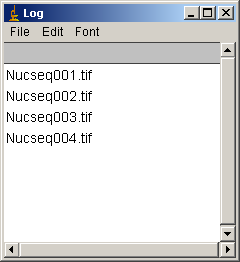
\includegraphics[scale=0.6]{fig/fig2521_FileBatchOUtput.png}
\caption{Output of code 22}
\label{fig:code22out}
\end{center}
\end{figure}

\begin{itemize}
\item Line 2: Asks the user to select a folder. Variable \ilcom{dir} is then stored with the full path to the folder. 
\item Line3 uses the \ilcom{getFileList} command, and reads out the file names as a string array and stored in List (array). 
\item Line 4 to 6 is a loop. \ilcom{list.length} returns the length of the list. In this way, all the contents are printed out in the window. 
We use this \ilcom{getFileList} command to process multiple files automatically. 
\end{itemize}

Let's modify code 22 so we can measure multiple stacks automatically. Code 23 (see below) works like this: You must first set two things: 

\begin{enumerate}
\item Full path to the destination folder where the results will be saved. 
Macro \ilcom{Set Directory to save Results}
\item Threshold level for the particle analysis. Macro \ilcom{set the threshold lower level}
\end{enumerate}

The first setting task is the same as you did in code 22. 
The second setting is done by manually opening a stack 
(may be the first one in the files) and manually setting the threshold as you like, 
then execute the second macro below. In both these settings, 
parameters will be saved in global variables and will be used in the main program. 

When you run the main macro (\ilcom{Multiple measurement}) 
after these two settings, the program asks you where the files are. 
As soon as you select a folder where files are contained, 
then processing and saving just proceeds automatically. 

\lstinputlisting[morekeywords={*, }]{code/code23_FileIO_02.ijm}

Now we have three macros and four global variables. 
\begin{itemize}
\item Line 3: global string variable for storing path to the source folder. 
\item Line 4: global string variable for storing path to the destination folder, where results will be saved. 
\item Line5 and 6: Global numerical variables for storing threshold upper and lower values. 

\item Macro \ilcom{Set Directory to save Results}: Line 9 to 12: First macro. This is used to set the path to the destination folder. The function is same as code 22.
 
\item Macro \ilcom{set the threshold lower level}: Line 14 to 20: 
This macro is for storing the lower value of the threshold in global variables, 
the values of which will be used in the main macro. You might have seen a similar code already: code 17, 
function for checking if the image is thresholded. 
Only difference is that in this code 23, 
lower threshold value is stored in the global variable defined in line 5. 
Upper value is not touched, kept to 255. 

\item Macro \ilcom{Multiple measurement}: Line 22 to 28: This is the main macro (third one in this macro set). 
Line 23 asks the user where the files are. 
This path to the source file is stored in the global variable defined in line 3. 
Then in line 24, a list of files contained in source folder is generated and stored in the array \ilcom{list}. 
From line 25 to 27 is a small for-loop, the number of loop is same as the length of the list. 
In this loop, name of file is passed one by one to the 
function \ilcom{NucAnalysis()} that does the actual analysis\ldots

\item function \ilcom{NucAnalysis(img\_filename)}: Line 30 to 51 is the core of analysis. 
\ilcom{img\_filename} is string variable for file names in the list array, given as argument. 
\begin{itemize}
\item Line 31: Using \ilcom{img\_filename},  the full path name is constructed by combining two strings. 
\item Line 32: A file is opened by \ilcom{open(path)} command. 
\begin{indentCom}
\textbf{open(path)}\\
Opens and displays a tiff, dicom, fits, pgm, jpeg, bmp, gif, lut, roi, or text file. 
Displays an error message and aborts the macro if the specified file is not in one of the supported formats, 
or if the file is not found. 
Displays a file open dialog box if path is an empty string or if there is no argument. 
Use the File>Open command with the command recorder running to generate calls to this function. 
With 1.41k or later, opens images specified by a URL.
\end{indentCom}
\item Line 33: After opening image, its \ilcom{ImageID} is stored in the variable \ilcom{sourceID}. 
\item Line 34, the image is thresholded according to the global variables for the lower and the upper values. 
\item Line 35: Title of the image, which actually is the file name, is retrieved and stored in the variable \ilcom{img\_title}. 
\item Line 38: The particle analysis is then applied to the image (Lines 34 to 37 are same as lines 14 to 17 in code 21). 
\item Line 38: Source image you opened from the hard disk is activated and then closed in line 39. 
Activation of the image by \ilcom{selectImage()} is required, 
because there is already a new stack (outline stack!), 
so that original stack is already behind. Therefore to close the original, 
one must activate the image by using \ilcom{selectImage()} command.  
\item After all these processing and measurement, results will be saved. 
Lines 42 to 45 saves the outline stack. Outline stack is also closed after saved (line 45). 
Line 47 to 50 is exactly same as the Result table saving you did in code 21 (lines 18 to 20). 
Line 49 is added, just for an additional information printout in Log window. 
\end{itemize}
\end{itemize}
\newpage
\section{Secondary Measurement}
In this section we learn a macro usage which you may often encounter in actual situations: 
We do certain measurement first. We then use results from this first measurement for 
setting parameters of second measurement.  

We take following example of secondary measurement: 
\begin{enumerate}
\item We first measure XY coordinates of moving particles by particle tracking.  
\item Using these XY data, we measure changes in pixel intensity of the particle.
\end{enumerate} 
There could be two cases of how you get the data out and load it into currently running macro. 
First is to do so directly from data table within ImageJ, 
and the other is to access data file saved in hard disk. We learn both. 

\subsection{Using Values in Results Window}

ParticleTracker is an excellent plugin for automated tracking of spherical particles\footnote{ As of Nov. 2010, we have a largely updated version of ParticleTracker plugin available at the ETH site. This 2D/3D implemented version could be downloaded from ETH site \url{
http://www.mosaic.ethz.ch/Downloads/ParticleTracker}.This plugin is added with many new features but there is some bugs still. With some measurement conditions, the new plugin returns error and crashes. For this reason, please download the plugin from CMCI site for the exercise in this textbook. \url{http://cmci.embl.de/downloads/particletracker2d}.  }. We use this plugin first to get tracked data. 

\begin{indentexercise}{1}
\item Open sample image stack \textbf{TransportOfEndosomalVirus.tif}. Then do \ijmenu{[Plugins > Particle Detector \& Tracker> Particle Tracker]}. A parameter input dialog window appears. Fill in  parameters as follows:
\begin{itemize}
\item radius: 3
\item cutoff: 0
\item percentile: 0.3
\item link range: 1
\item distance: 20
\end{itemize}
\end{indentexercise}

Now, you should see a results window that looks like figure \ref{fig:particletrackingresults}.
%figure 
\begin{figure}[htbp]
\begin{center}
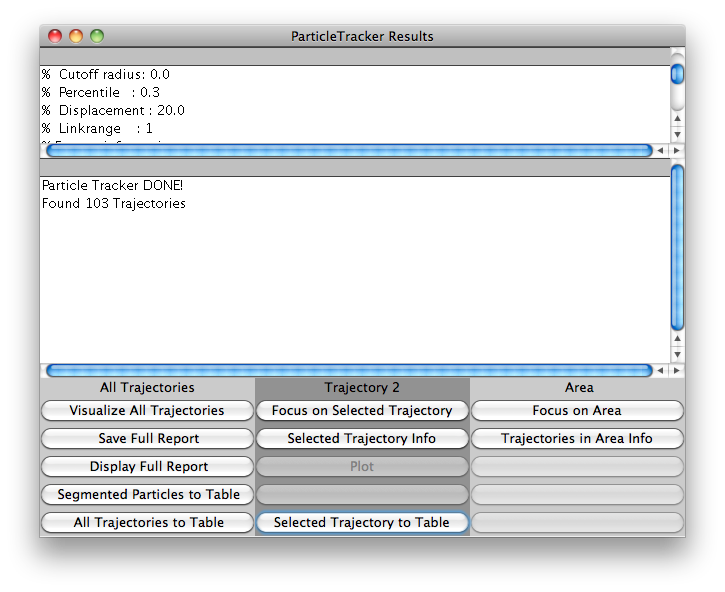
\includegraphics[scale=0.45]{fig/fig253_ParticleTrackerResults.png}
\caption{ParticleTracking Results}
\label{fig:particletrackingresults}
\end{center}
\end{figure}
In there, it should be reported that over 100 trajectories were detected. You could see how they look like by clicking "Visualize All Trajectories". 
Another window overlaid with colorful tracks appears 
(Fig. \ref{fig:particletrackingTracks}). 
Click "Filter Options" and input 10, so that short trajectories become invisible in the window. 
Use your mouse and select one of trajectory by clicking. 
Rectangle ROI is created in the surrounding of the selected track. 
Go back to the Results window (Fig. \ref{fig:particletrackingresults}) 
and click "Focus on Selected Trajectory". 
Then you will see another window is created with only the track you chose 
(Fig. \ref{fig:particletrackingTrackFocused}). 
Check carefully if the tracking was done properly. 
If you are satisfied, go back to the result window (Fig. \ref{fig:particletrackingresults}) 
again then click "selected trajectory to Table". 
You will then find the trajectory data is transferred to the Results table of ImageJ 
(Fig. \ref{fig:particletrackingTransferred}). 
 

%double figure
\begin{figure}[htbp]
 \centering
 \subfloat[]{\label{fig:particletrackingTracks}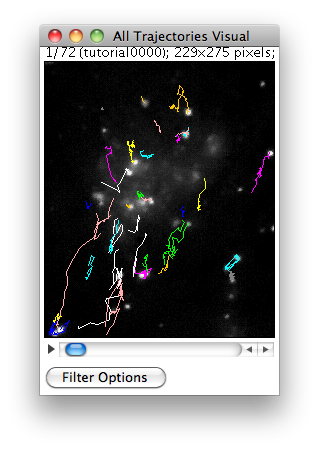
\includegraphics[height = 90mm]{fig/fig253particletrackingTracks.png}}
 \subfloat[]{\label{fig:particletrackingTrackFocused}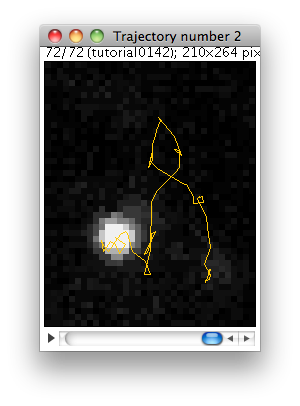
\includegraphics[height = 90mm]{fig/fig253_focusedTrajectory.png}}
 \caption{ (a) ParticleTracking Trajectories, all, and (b) Focus on Single Track.}
 \label{fig:particletrackingTrackFocused}
\end{figure}

 %figure 
\begin{figure}[htbp]
\begin{center}
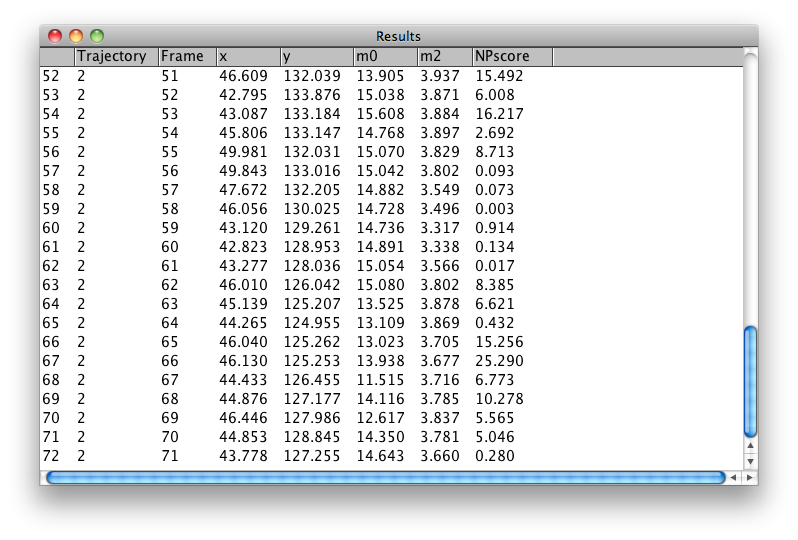
\includegraphics[scale=0.4]{fig/fig253_TrackingResultsInResultsTabel.png}
\caption{ParticleTracking Results transferred to ImageJ Results Table}
\label{fig:particletrackingTransferred}
\end{center}
\end{figure}

So now, what we have to do is access results table, 
get XY coordinates from there and do intensity measurements at corresponding positions. 
To get data out of results table, we use the following macro command:
\begin{indentCom}
\textbf{getResult("Column", row)}\\
Returns a measurement from the ImageJ results table or NaN if the specified column is not found. 
The first argument specifies a column in the table. 
It must be a "Results" window column label, such as "Area", "Mean" or "Circ.". 
The second argument specifies the row, where 0<=row<nResults. 
nResults is a predefined variable that contains the current measurement count. 
(Actually, it's a built-in function with the "()" optional.) 
Omit the second argument and the row defaults to nResults-1 (the last row in the results table). 
See also: nResults, setResult, isNaN, getResultLabel.
\end{indentCom}
Let's first test with a short macro that reads data from Results table and 
print out XY coordinates in the Log window. 

\lstinputlisting[morekeywords={*, getResult, nResults}]{code/code24.ijm}

At line 1, \ilcom{nResults} is a command that returns number of rows in the Results table. 
Frame number is added with 1 in the line 2  because frame number in ParticleTracker plugin starts from 0, 
while it starts from 1 in ImageJ. 
In line 3 and 4, xpos and ypos is inverted, 
because ParticleTracker program was originally wrote in Matlab and for that convention 
(in Matlab, vertical diretion is called "X" and horizontal direction is called "Y", 
and this is common to matrix calculation software since row = X and column = Y), 
XY data should be inverted for use in in ImageJ. 

If you check the log window and if you are confident with data read out from Results window, 
we could now add the code with lines to measure intensity by 
placing circular ROI at XY coordinates of trajectory. Here we go. 

\lstinputlisting[morekeywords={*, getResult, makeOval}]{code/code24_5.ijm}

Running this macro, you should see a new column in Results window with header title "RoiInt", 
where measured intensity is listed (Fig. \ref{fig:PTResultsTableAfter}).

%figure 
\begin{figure}[htbp]
\begin{center}
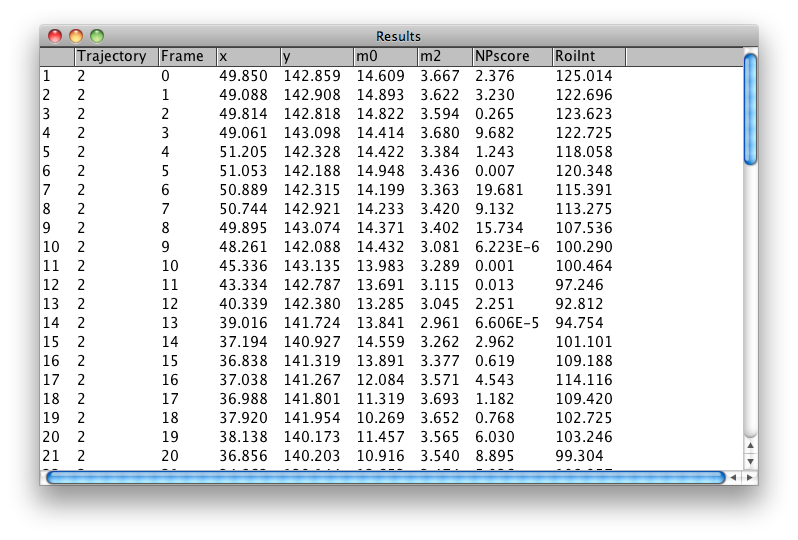
\includegraphics[scale=0.5]{fig/fig261_resultstableAddedWithInt.png}
\caption{Results Table with Intensity Measurement \\Column "RoiInt"}
\label{fig:PTResultsTableAfter}
\end{center}
\end{figure}

Explanation of the code: In the first line, 
we set the name of the image stack so that we are sure with which window to be measured with intensity. 
Line 2 and 3 are for setting the size of oval ROI. 

The way oval ROI is created is what you have learned already in detail in the section 
\ref{sec:dotmove}. \ilcom{getRawStatistics()} returns basic parameters of the selected ROI, 
and is more convenient than using \ilcom{run("Measure")}. 

\begin{indentCom}
\textbf{getRawStatistics(nPixels, mean, min, max, std, histogram)}\\
This function is similar to getStatistics except that the values returned 
are uncalibrated and the histogram of 16-bit images has a bin width of one and is returned 
as a max+1 element array. For examples, refer to the ShowStatistics macro set. 
See also: calibrate and List.setMeasurements
\end{indentCom} 

\subsection{Using values in non-Results table}
Next, we study a case when data are shown in non-Results Table. 
Manual Tracking plugin is another way of measuring particle movement, and utilizes non-Results table. 

\begin{indentexercise}{1}
Open sample image stack \textbf{TransportOfEndosomalVirus.tif} 
and track at least two virus manually\footnote{ For detailed instruction on how to use Manual tracker, 
see corresponding section in CMCI Image Processing and Analysis Course I Basic.}. 
In ImageJ, you should install this plugin by yourself. 
In Fiji, Manual Tracking plugin could be found at \ijmenu{[Plugins > tracking >]}.
\end{indentexercise}

After the tracking, we have a results table that looks like figure \ref{fig:manualtrackingresults}.
%figure 
\begin{figure}[htbp]
\begin{center}
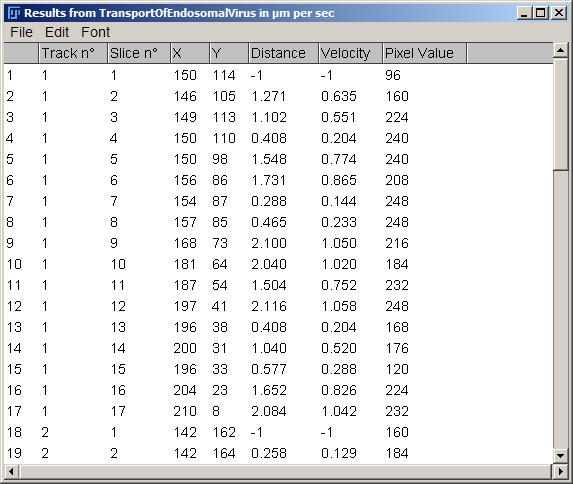
\includegraphics[scale=0.6]{fig/fig253_ManualTrackerResultsWindow.png}
\caption{Manual Tracking Results}
\label{fig:manualtrackingresults}
\end{center}
\end{figure}

To extract these data and use it for the secondary measurement, 
you might immediately think of using \ilcom{getResult(column header, row)} 
as we did in the previous subsection.

That should then be pretty straight forward\ldots 
But if you try this, you would see that this function returns error and 
does not work in case of Manual Tracking plugin. 
This is because result table created by Manual Tracking plugin is not the genuine ImageJ Results window. 
For such non-genuine results window, we retrieve data using the following command. 
\begin{indentCom}
\textbf{getInfo("window.contents")}\\
If the front window is a text window, returns the contents of that window. 
If the front window is an image, returns a string containing the text that would be displayed by 
Image>Show Info. Note that \ilcom{getImageInfo()} is a more reliable way to retrieve information 
about an image. Use \\
\ilcom{split(getInfo(),"\textbackslash{}n")} \\
to break the string returned by this function into separate lines. Replaces the \ilcom{getInfo()} function.
\end{indentCom}

This command returns a string with the content of the table. 
Try the following two lines to see how it works. \\

\begin{lstlisting}[numbers=none, morekeywords={*, getInfo}]
str = getInfo("window.contents");
print(str);
\end{lstlisting}
If you run these two lines, you will see data printed out in the Log window 
(Fig. \ref{fig:manualtrackingresultsLog}). 
%figure 
\begin{figure}[htbp]
\begin{center}
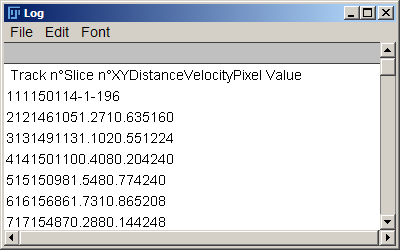
\includegraphics[scale=0.6]{fig/fig253_AllValuesinLog.png}
\caption{Manual Tracking Results in Log window}
\label{fig:manualtrackingresultsLog}
\end{center}
\end{figure}

So far so good, we succeeded in getting data out of the results table. 
Then what we need to do now is to play around with \ilcom{str} variable, 
where all the data is now contained as a chunk.  Since this chunk of data is not usable directly, 
we first split the \ilcom{str} to single lines of string array. 
For this we use \ilcom{split} command, the definition of which is 

\begin{indentCom}
\textbf{split(string, delimiters)}\\
Breaks a string into an array of substrings. 
Delimiters is a string containing one or more delimiter characters. 
The default delimiter set " \textbackslash{}t\textbackslash{}n\textbackslash{}r" 
(space, tab, newline, return) is used if delimiters is an empty string or split is called with only one argument. 
Returns a one element array if no delimiter is found. 
\end{indentCom}

Using this command to convert the string to a string array and adding two more lines to check the content of array, 
code now looks like this:\\
\begin{lstlisting}[numbers=none, morekeywords={*, split}]
str = getInfo("window.contents");
//print(str);
strA = split(str, "\n");
print(strA[0]);
print(strA[1]);
\end{lstlisting}
We use delimiter \ilcom{\textbackslash{}n} which means "new line", a hidden command in \ilcom{str} 
that feeds new line to form a table. When we run above code we will see two data shown in the log window (Fig. \ref{fig:splittedLine}).
%figure 
\begin{figure}[htbp]
\begin{center}
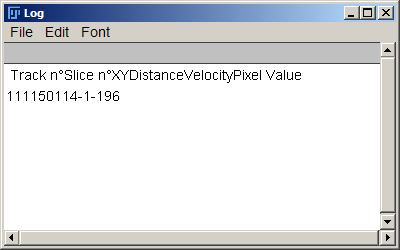
\includegraphics[scale=0.6]{fig/fig253_ZeroAndfirstlineValues.png}
\caption{Two Lines from data in the Log window}
\label{fig:splittedLine}
\end{center}
\end{figure}

We then still need to split each single line to individual data for each column. We modify the code as follows:
\begin{lstlisting}[numbers=none, morekeywords={*, split}]
str = getInfo("window.contents");
strA = split(str, "\n");
lineA = split(strA[1], "\t");
print(lineA[3]);
\end{lstlisting}

We use delimiter \ilcom{\textbackslash{}t}, which means "tab", to convert single line to an array of data. each for a column. 
%figure 
\begin{figure}[htbp]
\begin{center}
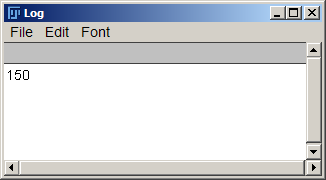
\includegraphics[scale=0.6]{fig/fig253_XfirstlineValue.png}
\caption{Elementary data in the Log window}
\label{fig:doublesplittedLine}
\end{center}
\end{figure}

The value shown in the Log window (Fig. \ref{fig:doublesplittedLine}) 
should be the same as X value in the first row of the original table (Fig. \ref{fig:manualtrackingresults}). 

We now know how to access individual data values within \ilcom{str}, 
by first splitting it with delimiter  \ilcom{\textbackslash{}n} and then by  
\ilcom{\textbackslash{}t}. We can print all XY coordinates in Log window by following code.  

\lstinputlisting[morekeywords={*, split}]{code/code25.ijm}

If you encounter error message with \ilcom{lineA[]} such as shown in fig.\ref{fig:fig262_ErrorMessage}, 
this is just because there is another text widow opened and \ilcom{getInfo()}command worked on 
that window rather than the results table of the Manual Tracking. To avoid such error, 
close extra text windows and then try running the macro again. 
%figure  
\begin{figure}[htbp]
\begin{center}
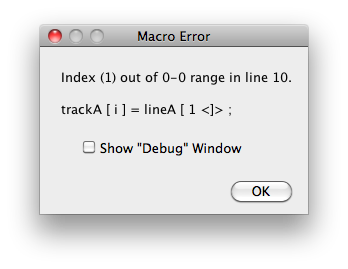
\includegraphics[scale=0.6]{fig/fig262_PossibleErrorMessage.png}
\caption{Possible Error Message with Code25 and Code25.5}
\label{fig:fig262_ErrorMessage}
\end{center}
\end{figure}

From line 4 to 7, new arrays are generated to store data from four columns in the for-loop from line 8 to 14. 

%figure  
\begin{figure}[htbp]
\begin{center}
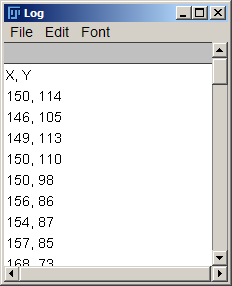
\includegraphics[scale=0.6]{fig/fig253_CoordinatesPrintedOut.png}
\caption{Elementary data in the Log window}
\label{fig:fig253_CoordinatesPrintedOut}
\end{center}
\end{figure}

Check the log window (Fig. \ref{fig:fig253_CoordinatesPrintedOut}), 
compare the output with manual tracker results table, and if you are confident that you are accessing data in table, 
you could then use XY coordinates to place a circular ROI, 
measure average intensity in that area and list them in ImageJ Results window.

\lstinputlisting[morekeywords={*, split}]{code/code25_5.ijm}

Running this code, you should see Results window that looks like figure 
\ref{fig:fig262_ManualTrackIntfinalResults}, tracking data plus measured intensity is shown in 
column titled "RoiInt". The way oval ROI is used to measure mean intensity is similar to what 
we have coded in the previous subsection. A difference is that this time, we use arrays that store data 
extracted by splitting the chunk of string data. 

%figure  This should be replaced with results window!!!
\begin{figure}[htbp]
\begin{center}
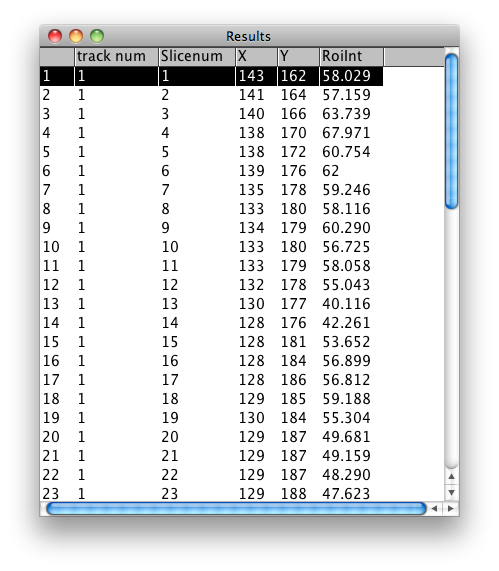
\includegraphics[scale=0.5]{fig/fig262_ManualTrackIntensityFinalResults.png}
\caption{ Manual Tracker Results in IJ Results table\\ now with measured intensity column RoiInt}
\label{fig:fig262_ManualTrackIntfinalResults}
\end{center}
\end{figure}

We then successfully measured the intensity dynamics of moving object again.  

\newpage
\subsection{Accessing Data File: Simple Case}
In this section and in the next section, 
we study how to access data in saved file for secondary measurements. 

Two cases we studied so far were both accessing data listed in a table that is already loaded in ImageJ 
(data is already an instance of ImageJ). What if we want to use data that is saved as a file? For example, 
we want to use results of Manual Tracking (previous section) that was saved as an .xls file and 
you want to use its data for secondary measurement. More generally, you did particle tracking using different software 
such as Imaris Track, and you want to use  coordinate data from that analysis for intensity measurement to be done in ImageJ. 
In such cases, we should access tabulated data in file accessing from ImageJ. 

In this section, we try accessing data saved by Manual Tracking. 
Loading data file could be done by a small modification 
of the code we studied in the previous section. Instead of command 
\ilcom{getInfo("window.content")} in line 3 of code 25.5, we use \ilcom{FileOpenAsString(path)} to retrieve 
file content into a string variable.  By leaving the argument \ilcom{path} blank (""), user will be asked for choosing a file. 
Since this is a simple one-line replacement of line 3 of code 25.5, below is the new code but only showing its first 10 lines.  

\lstinputlisting[linerange={1-10}, morekeywords={*, File, openAsString}]{code/code26.ijm}

To run this macro, be sure that you have your stack already opened, as it is required for measuring intensity. 

\subsection{Accessing Data File: Complex Case}

We now try making use of data file with more complex format. 
In the case we studied with Manual Tracking plugin in the previous section, data format was pretty straight forward 
so we did not have to do much work for dealing with the data format. 
In general, things are not so simple and one must figure out some way to decode the format for using it in secondary measurement. 

Automatic tracking plugin "ParticelTracker" allows you to save trajectory data by "Save Full Report" 
button in the results interface (see Fig. \ref{fig:particletrackingresults}). 
We try to access this data. 
\footnote{ This technique is especially important if you want to do automated particle tracking of many data. 
A new feature in ParticleTracker plugin released in Nov. 2010 is that when ParticleTracker is called from macro, 
it automatically saves data in folder where the image file is located. We then are able to process many files using macro, 
even recursively, and get tracking data automatically. For this reason technique for accessing ParticleTracker data file is valuable.}

First, you must prepare the data file. 

\begin{indentexercise}{1}
\item Open sample image stack \textbf{TransportOfEndosomalVirus.tif}. 
Then do \ijmenu{[Plugins > Particle Detextor \& Tracker> Particle Tracker]}. 
An interface appears, so fill in the parameters as follows:
\begin{itemize}
\item radius: 3
\item cutoff: 0
\item percentile: 0.3
\item link range: 1
\item distance: 20
\end{itemize}
\item Click "Save Full Report" and save the data file in the folder where sample image stack 
"\textbf{TransportOfEndosomalVirus.tif}" is. 
Saving dialog will come up with a proposal of file name to be "Traj\_<filename>.txt" 
so do not change that and simply click Save (this file name will be important). 
Close the Results interface. Do not close the image stack \textbf{TransportOfEndosomalVirus.tif}, 
as we will use it still in the following.
\end{indentexercise}

Now you are ready with data, so we try loading data into ImageJ/Fiji. Run the following code. 

\lstinputlisting[morekeywords={*, substring, lengthOf,File, exists, openAsString}]{code/code27_PTfileaccess.ijm}

You now have all the values in the log window, that should look like fig. \ref{fig:fig264_PTdatainLogWin}. 

%figure  
\begin{figure}[htbp]
\begin{center}
\includegraphics[scale=0.5]{fig/fig264_PTdataLoadedtoLog.png}
\caption{ ParticleTracker data loaded to Log Window}
\label{fig:fig264_PTdatainLogWin}
\end{center}
\end{figure}

Before getting into data file structure, let's look at what we have done in the code above. 
You might then study about how to deal with string, extracting parts of it. 
\begin{itemize}
\item Line 2: \ilcom{getDirectory} command with option \ilcom{("image")} 
will return a path of the last-opened image location. 
This will be where the file "\textbf{TransportOfEndosomalVirus.tif}", inside the sample image folder. 
\item Line 3: Filename of the image  "\textbf{TransportOfEndosomalVirus.tif}" is acquired. 
\item Line 4: Generating the file name of the data file. "Traj\_" is the prefix that was automatically added to 
the data file name. Command \ilcom{substring} extracts part of the string variable, and in our case, 
we try to get the image file name without ".tif". Definition of \ilcom{substring} command is as follows.

\begin{indentCom}
\textbf{substring(string, index1, index2)}\\
Returns a new string that is a substring of string. The substring begins at index1 and extends to the character at index2 - 1. 
See also: indexOf, startsWith, endsWith, replace.
\end{indentCom}

index1 should be 0, as we want from the beginning of the file name, and index2 should be 4 strings before the 
last string so we need the total length of the string. For this we use \ilcom{lengthOf} command. 
\begin{indentCom}
\textbf{lengthOf(str)}\\
Returns the length of a string or array.
\end{indentCom}
In this way, we construct the file name we want to access 
(the name of which originally is automatically generated when saving the data in Particle Tracker interface) 
the file further setting the full path to the file in line 5. 
\item Line 8: This line checks if the file full path generated above is valid. 
\ilcom{File.exists(full-path-to-file)} returns false if there is no such file. In that case, we should not proceed more so macro terminates at line 8. 
\item Line 11: If everything is ok, then the file is opened as a string, 
and the string will be printed in Log window by line 12. 
\end{itemize}

ParticleTracker data file consists of three parts. 
\begin{enumerate}
\item Header: contains information on the condition of tracking. 
\item Detected Particles: Detected particles in each frame is listed.
\item Trajectories: Trajectories are listed, one by one. 
\end{enumerate}
Since we need to access trajectory information, we need to go through the data string to reach the third part of the data structure. 
To do so we split the file by lines (\textbackslash{}n), then loop through the array to find the position where the trajectory information is contained. 

We examine the data file in detail, to see what could be the marker for the starting and end point of each trajectory. 
Here is a part of data, that is a directly copy and pasted below. 
\begin{lstlisting}[numbers=none]
24 154.894485 137.063614 7.338140 3.316167 15.683273
25 154.217377 138.368927 7.087145 3.417947 0.188002

%% Trajectory 37
15 22.111439 204.511826 9.726052 3.180977 28.252821
16 8.837964 209.618210 13.082743 3.273177 29.163294
17 0.432002 208.377045 3.574241 1.552869 0.000000
18 2.150804 209.609573 11.131773 2.939974 13.455443
19 10.542578 206.151169 14.173851 3.202391 14.258223
20 9.727753 206.960999 14.360144 3.250930 6.493425
21 15.708366 207.058640 14.943080 3.121640 0.053831
22 26.715679 208.680145 14.648912 3.091611 1.570746
23 29.143650 208.706314 13.616717 2.975144 21.279413
24 28.148304 202.200867 12.116886 2.862307 6.292521

%% Trajectory 38
15 142.326370 81.088326 5.813046 2.967546 13.995440
\end{lstlisting}
Single trajectory data start with a line with "\%\%Trajectory " plus numbering, and ends with a blank space. 
We use these information as markers for determining the location of trajectory data within file. Each line of data consists of 6 numbers: 
\begin{enumerate} 
\item Frame number
\item Y coordinate
\item X coordinate
\item image moment m0
\item image moment m2
\item Non-Particle Discrimination Criteria
\end{enumerate}
These values are separated by space. So splitting single line to an array of elementary data needs to be done by \ilcom{split(line, " ")}.

Here is a macro, that uses \ilcom{File.openAsString("")} to load the file and then loads the trajectory information 
into Results table with the strategy explained above. 

\lstinputlisting[morekeywords={*, }]{code/code28.ijm}

In the code 28, core of the processing resides within the function \ilcom{Load2ResultsV3}. 
It takes path to the data file and file name as arguments, and first opens the file as string at line 15. 
The chunk of string is then split by lines and for-loop starts to go through the array of lines (line 19). 

In every line in the array, if the line is a starting marker "\%\% Trajectory <number>" is tested (line 22) . 
If that is the case, then do-while loop is started, that loops until all the trajectory points are read out (line 24 to 41). 
While this trajectory read out is done, counter for the for-loop \ilcom{i} 
is also incremented that when the do-while loop ends (line 25), the for-loop starts again from the 
line after the data of that trajectory. Exit from do-loop occurs when blank line is found (line 42). 

Inside the do-while loop, space character is replaced with tab delimiter (line 26 to 32). 
This is required, since ImageJ results importing only recognized tab-delimited file as a table.  

There is a small adjustment by another function \ilcom{CommaEliminator} at line 32. 
This is required for removing comma character in some cases (this happens when the data file was opened and saved in excel or so). 
You probably do not need this line and function as we are using the data file directly after saving them. I left it in the code for your future usage. 

Just to be sure with data content, line 33 and 34 double-check that the line indeed contains several data. 
Line 35 to 38 writes trajectory ID, Frame number and XY coordinates into Results window by \ilcom{setResult} command.

\begin{indentexercise}{2}
\item Finally, we can combine several macros and functions we studied so far to make a new macro 
that loads the ParticleTracker data file to Results table, and read out intensity. 
This could be done by combining following codes, with a bit of modifications with each. 
\begin{itemize}
\item code 27 (check the current image stack name and loads its track data file as string)
\item code 28 (data in string format is converted to Result table)
\item code 24.5 (measure intensity according to coordinates in Results table)
\end{itemize}
Bits and pieces are already there. Please try completing a macro that loads track data file according 
to the title of the image stack that is already opened, place them in Results table, and then measure 
the intensity in corresponding frame and position in the image stack. 
\end{indentexercise}

\newpage

\section{Using Javascript}

As you become experienced with coding in ImageJ macros, you might start to find
out that for whatever you want to do with ImageJ, 
corresponding macro function does not exist in the Build-in Macro Functions page
\footnote{ see \url{http://rsb.info.nih.gov/ij/developer/macro/functions.html}}. 
One way to supplement the missing function is to create your own user function. 
Another way is to find a function directly from ImageJ Java code and use that function in macro. 
Javascript is a convenient way to access ImageJ API (Application Programming Interface), 
and since Javascript could be called from within ImageJ macro, you could use ImageJ API in your macro code. 
This is done by the macro function shown below:
\begin{shaded}
\begin{indentCom}
\item \textbf{eval("script", javascript)}\\
Evaluates the JavaScript code contained in the string javascript.\\
\end{indentCom}
\end{shaded}

This would be the simplest way to use Javascript if you are already
comfortable with ImageJ macro language. 

\textbf{But there is more to it}. You could also run Javascript as it is in
ImageJ and Fiji. Syntax of Javascript is not same as ImageJ macro, 
but if you are used to write ImageJ macro, it should not be too difficult to learn Javascript.  
 
\dots then how could we code Javascript? 

In this section, we learn basic know-how of 
Javascript with ImageJ 
\footnote{ If you want to learn in more detail, 
you could also visit \url{http://pacific.mpi-cbg.de/wiki/index.php/Javascript_Scripting} 
for learning more about Javascript.}. Experience with 
Java programming is largely helpful but if not, there is also some way around
to learn quickly. 

When we are programming ImageJ macro, we often refer to the
web site listing ImageJ macro language functions to look for a macro command. 
In similar way, we access so called API (Application Programming Interface) 
for coding with Javascript. ImageJ API is in the following page:

\url{http://rsb.info.nih.gov/ij/developer/api/index.html}

At this moment, you might be puzzled with these pages, 
but don't worry. Major aim of this section is to learn how to use this resource 
to code your Javascript. 

OK, let's start. 

\subsection{A trial with Javascript commands}
%
Let us first try using Javascript (JS) commands. 

From menu, do \ijmenu{[Plugins > Scripting > Javascript Interpreter]}. 
You will then see a new interface that looks like Fig \ref{fig:JSinterpreter}. 
This interface provides Javascripting in an interactive mode and is useful for 
a quick testing of codes. There is a input field at the bottom, where you could type in JS code. 
Then by pressing return key, the code is executed.  

\begin{figure}[htbp]
\begin{center}
\includegraphics[width=100mm]{fig2/JSinterpreterStasrtUp.png}
\caption{Javascript interpreter on start up.}
\label{fig:JSinterpreter}
\end{center}
\end{figure} 

Type the following command and execute by return key. 
\begin{lstlisting}[numbers=none]
IJ.log("Hello JS")
\end{lstlisting}
This JS command will print "Hello JS" in the Log window of ImageJ.  

Same command could be written in the Script editor. To start up the editor, 
do \ijmenu{[File > New > Script]} (then select \ijmenu{[Language > Javascript]}). 
\begin{lstlisting}[numbers=none]
IJ.log("Hello JS");
\end{lstlisting}
This should do the same thing, but be careful! Do not forget adding semicolon
(;) at the end of the line. In case you write your code in Script Editor, you need
to explicitly mark the end of line, just like you do when you write a macro.

To run the code, \ijmenu{[Run > Run]} will execute the command (you could also
use ctrl-r or cmd-r). 

What this JS code does is the same as the Macro code below. 
\begin{lstlisting}[numbers=none]
print();
\end{lstlisting}

In the following, you could use either Javascript interpreter 
or Script editor. Just choose the one you like. If code become multiple lines, 
I recommend you to use the Script Editor\ldots and in this case, this is a
redundant warning, place a semi-colon ``;'' at the end of each line.

Now, we could try some commands that is not present in 
ImageJ macro.
 
For example, what would you do if you want to convert angle in degrees to radian? 
In macro, you could do calculation by first dividing the value by 360, 
then multiply by $2\pi$. But a function actually is already there in Java, 
so you could simply use that as well. 
\begin{lstlisting}[numbers=none]
IJ.log(java.lang.Math.toDegrees(3.1415)) 
\end{lstlisting}
Running this line should print a number close to 180. You could also do the
other way around:
 \begin{lstlisting}[numbers=none]
IJ.log(java.lang.Math.toRadians(180)) 
\end{lstlisting}
should print out 3.1415\dots.

Next, we try to retrieve a column of data from table in Results window. 
In macro, you could do this by \ilcom{getResult} function, 
with which by specifying the column label and row number you could retrieve 
a value in that cell. 

But what should we do if we want to retrieve all data in a row at once, 
not a single value in a specific column at specific row? 
If you want to do this in macro, we could write a user defined function that loops 
for all the columns and get data one-by-one. 

With Javascript, this could be done in just a single step, one command. 

\begin{indentexercise}{1}

\textbf{Preparation of Results table}

Open image by \ijmenu{[File > Open Sample > blobs (25k)]}. 

Check measurement parameters by 

\ijmenu{[Analyze > Set Measurements\dots]}

that some measurement parameters are checked. Be sure that "Limit to Threshold" is checked. 

Then Threshold the blob image by 

\ijmenu{[Image > Adjust > Threshold]}. 

Since the background of this image is bright, Dark Background' should be unchecked. 
If you see the thresholded image like fig. \ref{fig:ThresBlob},  do 

\ijmenu{[Analyze > Analyze Particles\dots]}. 

%figure
\begin{figure}[htbp]
\begin{center}
\includegraphics[height=50mm]{fig2/ThrehsoldedBlob.png}
\caption{Thresholded image of "blob"}
\label{fig:ThresBlob}
\end{center}
\end{figure} 

In the Analyze Particles dialog, just be sure that \textbf{Display Results} is checked. 
Then click OK button. When the analysis is done, you will see  64 or so particles detected 
and listed in the Results window. 

\textbf{Testing Javascript Code}

We now use the following command to extract data from single Row. In Javascript
interpreter, type the following command .

\begin{lstlisting}[numbers=none]
IJ.log(ResultsTable.getResultsTable().getRowAsString(10));
\end{lstlisting}

If you execute this, you will see that all data that is in row 11 in Results table is 
now printed in the log window. 

\dots that's the end of this exercise but don't close the Results window yet.   
\end{indentexercise}

Above is a single line pure JS code. 
We can use this code within macro by using \textbf{eval} function mentioned already. 
Here is an exercise to test the function \textbf{eval}. 

\begin{indentexercise}{2}
Test running the following code, and check that any row in the table could be extracted 
and printed in Log window. 
\begin{lstlisting}
rownum = getNumber("Row?", 0);
jscom = "IJ.log(ResultsTable.getResultsTable().getRowAsString("+rownum+"));";
eval("script", jscom);
\end{lstlisting}
\end{indentexercise}

In the second line, JS code is constructed as a single string \ilcom{jscom} 
using the variable \ilcom{rownum} from line 1. Line 3 executes this JS code using \textbf{eval}. 

So far, I have not yet explained where these commands came from. 
I will give more detailed explanation in later sections.  

\begin{indentexercise}{2}
This exercise is optional:

Try the following Javascript commands using \textbf{eval}, from within an ImageJ
macro.

\dots lists all ImageIDs. There should be at least one image opened. 
\begin{lstlisting}[numbers=none]
a = WindowManager.getIDList();
for(i in a) IJ.log(a[i]);
\end{lstlisting}

\dots zooms current image centered at top-left corner.
\begin{lstlisting}[numbers=none]
IJ.getImage().getCanvas().zoomIn(0, 0);
\end{lstlisting}

\dots print souts statistics of current image in log window.
\begin{lstlisting}[numbers=none]
eval("script", "IJ.log(IJ.getImage().getStatistics().toString());");
\end{lstlisting}

\dots print outs used memory in log window.
\begin{lstlisting}[numbers=none]
eval("script", "print(IJ.currentMemory())");
\end{lstlisting}

\dots moves current image window to top-left corner of the monitor with offset of 10 by to, 
and resizes the window. 
\begin{lstlisting}[numbers=none]
eval("script", "IJ.log(IJ.getImage().getWindow().setLocationAndSize(10, 10, 100, 100))");
\end{lstlisting}
\end{indentexercise}

In all the example codes, we placed Javascript commands in the second argument 
for the function \textit{eval}. 
You could also write a full path to a Javascript file. Here is the syntax. 
\begin{shaded}
\begin{indentCom}
\item \textbf{eval}('script', \textbf{File.openAsString}("<pathpath>/name.js")) ;
\end{indentCom}
\end{shaded}

\subsection{Using Macro Recorder and ImageJ API}
Javascript is a scripting language, so it has its own build-in functions. 
I will not explain about this since you could find many Javascript tutorials on the web. 
For example, following site is a place where I go and look for Javascript commands and usages:

\href{http://www.w3schools.com/jsref/default.asp}{Javascript Reference @ w3chools.com}

How do we find Javascript commands to interact and control ImageJ? 
The easiest way is to use the macro recorder. 
We have already learned and used macro recorder in previous chapters. 
We could used the same interface for recording JS codes. 
Recorded lines of JS codes could be copy \& pasted into Script Editor and can be directly executed. 

\begin{indentexercise}{1}
First, we should start the recorder. 
\ijmenu{[Plugins > Macros > Record\dots]}. 
Then in the recorder window at the top-left corner, 
choose Javascript as the code to be recorded (Fig. \ref{fig:MacroRecorderJS}). 

%figure
\begin{figure}[htbp]
\begin{center}
\includegraphics[width=70mm]{fig2/RecorderJS.png}
\caption{Setting Up Macro Recorder ready for Javascript}
\label{fig:MacroRecorderJS}
\end{center}
\end{figure}

Then do the following sequence of commands.
\begin{itemize}
\item \ijmenu{[File > Open Sample > Blobs]}
\item Select rectangular ROI tool and set a ROI to select 
about 1/4th of the image (can be any place within the image. This is just a test.). 
\item \ijmenu{[File > Transform > Flip Horizontally]}
\item \ijmenu{[Process > Filters > Gaussian Blurr\dots]}
\end{itemize}
After all these operations, there should be JS codes printed in the Recorder window. 
Copy them all, and paste it to Script Editor (\ilcom{[File > New > Scripts]} and then paste, 
Fig. \ref{fig:ScriptEditorRecorded}) . 
After pasting, set language to JS by (\ilcom{[Language > Javascript]} from the menu bar of script editor.  

%figure
\begin{figure}[htbp]
\begin{center}
\includegraphics[height=50mm]{fig2/JSrecordedInScriptEditor.png}
\caption{Javascript by recorder commands.}
\label{fig:ScriptEditorRecorded}
\end{center}
\end{figure}

Then do \ilcom{[Run > Run]} from the menu of script editor, the script is executed. 
You should then see a new window of "blob" with some part of image processed. 
\end{indentexercise}
If you are successful in running the code, let's see the code. Here is how the code should look like. 

%\lstinputlisting[morekeywords={*}]{code/code29.js}
\lstinputlisting{code/code29.js}

We first examine line 3 and line 4, focusing on the method \ilcom{IJ.run}  
(in the follwoing, we use word "method" instead of "command", as this is more 
conventional way of calling it in Java). This method has three arguments for it.

\ilcom{IJ.run(argument1, argument2, argument3)}

 Just by looking at each of them you could realize that the second argument 
 is a descriptive explanation of what the method does. 
 This is because these strings are exactly the phrase of the menu item you see 
 when you choose that function from ImageJ menu. 

\ilcom{IJ.run} is a method that uses second argument as a keyword 
to search for all the ImageJ menu items to find which of them is the one 
that the method intends to invoke 
\footnote{In ImageJ macro, a function similar to \ilcom{IJ.run} 
method is \ilcom{run(arg1, arg2)}.}. 
Third argument of \ilcom{IJ.run} in line 3 is an empty string, 
but in line 4, the third argument is \ilcom{sigma=2}. 
This is a value that you normally input when you select Gaussian blur 
from the menu bar for the size of blurring kernel. 

Then what is the first argument in \ilcom{IJ.run}? 
In both line 3 and 4, we have a variable \textbf{\ilcom{imp}}. 
To see what this is, we go back to line 1. 
\textbf{\ilcom{imp}} appears for the first time in the code at line 1, 
and \textbf{\ilcom{imp}} is the returned value of a method \ilcom{IJ.openImage}. 
If we think back what we were actually doing for this first line when recording, 
we accessed an item in the menu tree \ijmenu{[File > Open Sample > blobs]}. 
By choosing this item from menu, ImageJ downloads blobs.gif file from NIH web site 
and then shows it on your desktop. 
Single method that does the download action is the method \ilcom{IJ.openImage}. 
Argument for this command is the URL of the image. 

To know the definition of the method \ilcom{IJ.openImage}, 
we look up a reference called 
\href{http://rsb.info.nih.gov/ij/developer/api/index.html}{ImageJ API}
\footnote{ ImageJ API: http://rsb.info.nih.gov/ij/developer/api/index.html}. 
In this web page, there is side bar in left side, with upper part 
for a list of "All Packages" 
(These packages are same as those listed in the table shown in the top page) 
and the bottom part for "All Classes".  

%figure
\begin{figure}[htbp]
\begin{center}
\includegraphics[height=75mm]{fig2/IJAPItop.png}
\caption{ImageJ API}
\label{fig:IJAPItoppage}
\end{center}
\end{figure}


Each package contains several classes. 
We currently do not know which package does 
\ilcom{IJ.openImage} belong to, so we look for it in the bottom part "All Classes". 
There, you will find "IJ"\footnote{ Unlike ImageJ macro, Java and Javascript are case sensitive}. 
Click the link, and in the right side of the page, a page titled "Class IJ" appears 
(Fig. \ref{fig:IJAPClassIJ}). 

%figure
\begin{figure}[htbp]
\begin{center}
\includegraphics[width=75mm]{fig2/IJAPI_IJ.png}
\caption{ImageJ API Class IJ}
\label{fig:IJAPClassIJ}
\end{center}
\end{figure}

The page might look cryptic to you, if you scroll down the page, there is a table titled "Method Summary", listing all the methods that class IJ contains in alphabetical order. 
Within this list, you will find (Fig. \ref{fig:IJAPIIJopenImage})

\ilcom{openImage(java.lang.String path)} 


%figure
\begin{figure}[htbp]
\begin{center}
\includegraphics[height=75mm]{fig2/IJAPI_IJopenImage.png}
\caption{ImageJ API Class IJ, openImage method}
\label{fig:IJAPIIJopenImage}
\end{center}
\end{figure}

There are three \ilcom{openImage} methods, with difference in number and types of arguments. 
The first one is without any argument, the second one has only one argument, 
the third having two arguments. 
When openImage method is called, one of these three are called depending on the number 
and types of the argument in the call. 

\textbf{More Explanation:} So what are "Classes?" A class consists of two major components. 
One is Field and the other is Method. 
The former is like variable and the latter is similar to function in ImageJ macro 
(this is not a precise analogy, but for now let's think like that). 
Fields are values. Methods are actions. Class is a group of various field values and methods. 
By utilizing Class, we can have a single unit of assembled functions, 
which would be an advantage for letting an application to have high modularity. 
You could access (or use) fields and methods by appending them behind the name
of the class. For example. <class name>.<field name> or <class name>.<method name>(<arguments>) 
e.g. \ilcom{IJ.openImage(pathname)}.

 \textbf{A bit more on API page} At the top of the Class IJ page (Fig.\ref{fig:IJAPClassIJ}), 
 "ij" is written above the class name "Class IJ". 
 This is the name of package that is containing this class. 
 You could see all classes within the package ij (note: case sensitive), 
 click "ij" in the left top panel listing "all packages".  
 You then will see all the classes within the package ij, 
 such as compositeImage, Executor, IJ, ImageJ\dots and so on. 
 Package is used to organize classes in hierarchical tree. 
 For example, there are packages ij.plugin, ij.plugin.filter and ij.plugin.frame. 
 Likewise, package is a tree-like structure (remember how folders are organized in your laptop) 
 that organizes many classes in a structure. In Java, such tree-like structure
 is organized separated by dots (``.''). For example, see
 \href{http://rsb.info.nih.gov/ij/developer/api/ij/plugin/filter/package-summary.html}{Package
 ij.plugin.filter}. The package filter is under the plugin package, that is
 under the ij package. 
  
Go back to the API description, in the left side of the table column where 

\ilcom{openImage(java.lang.String path) } 

is listed (Fig. \ref{fig:IJAPIIJopenImage}), there is a phrase 

\ilcom{static ImagePlus} 

This tells you that if you invoke method \ilcom{openImage(java.lang.String path)} of class \ilcom{IJ}, 
a object called ImagePlus is returned (forget about the notion "static" for now). 
ImagePlus is another class, which you could also look up using the list of "All Classes".  

The class ImagePlus consists of image data and metadata fields, and methods to access these values. 
In \href{http://rsb.info.nih.gov/ij/developer/api/ij/ImagePlus.html}{ImagePlus API page}, 
you could see that many fields and methods are associated with this class. 
Note that many of field values are "protected". 

For example, \ilcom{nChannels} is one of the filed values of class ImagePlus 
but having a notion "protected" means that you cannot simply access from outside the class itself. 
Instead, there is a method named \ilcom{getNChannels()} for accessing the value 
from outside which by invoking it "Returns the number of channels" of ImagePlus object. 
\ilcom{getNChannels()} returns a value indicated as "int". 
This tells you that the type of returned object is "int", which means that returned value is a number, 
and specifically an integer, not a number with decimal points. Unlike ImageJ macro 
\textbf{object} with any type of class could be returned, not limited to number, string and array. 
This flexibility affords higher potential in modularity with Javascript compared to ImageJ macro 
and hence we call returned values as "object" not "variables". 

A draw back is that Javascript coding becomes a bit more complicated then macro
coding. One should always be careful about which class or type is returned, 
and one way to do so is to check ImageJ API every time you wonder what is the
returned value of certain method.

Let's go back to the code again. 
The method \ilcom{IJ.openImage} returns an \textbf{object "ImagePlus"}, 
so in line 1 of the recorded Javascript code, 
an instance of ImagePlus object (which actually is "blob.png" downloaded from the NIH website) 
is stored in the variable "imp". 
Then after line 1, \ilcom{imp} behaves as an ImagePlus object. 
\ilcom{imp} is repeatedly used from line 2 to 5. In line 2, an method of class ImagePlus is invoked 
in the form <class>.<method>(arguments). 
Since method name is \ilcom{setROI} we look for it in the 
\href{http://rsb.info.nih.gov/ij/developer/api/ij/ImagePlus.html}{ImaegJ API ImagePlus page}, 
and you will find the following description:

\begin{quote}
void | setRoi(int x, int y, int width, int height) \\
          Creates a rectangular selection.
\end{quote}

"void" means that this method does not return any value. 
There are four arguments and all of them are "int", integer. 
Description tells you that this methods creates an ROI in the image with position and size 
defined by arguments.  

In line 3 and 4, the first argument of \ilcom{run} method is \ilcom{imp}, 
telling the command \ilcom{IJ.run} to do the operation specified by the second argument on \ilcom{imp}. 

Note that in case of ImageJ macro, target image could only be specified by 
activating the window using \ilcom{selectImage(imageID)}. 
In Javascript, selection of image could be more explicit by the direct use of ImagePlus object.  

Down to line 4, blob image actually is not shown on the desktop. 
ImagePlus object of "blobs.tif" is in the memory, but still is not displayed. To
show it on the desktop, we do line 5.

\begin{quote}
\ilcom{imp.show();}
\end{quote}

\ilcom{show()} is a method of ImagePlus class to show the actual image of ImagePlus object. 

%In case of Macro, we could execute that as a single line. 
% So how about doing the same? 
% Create a new script tab by \ijmenu{[File > New]} 
% from the script editor menu. 
% Then copy line 4 and paste that single line in the new script.

\textbf{Grabbing Image}
What if you want to capture already opened Image as a ImagePlus object? 
This could be done by using a method in Class IJ called \ilcom{getImage()}. 
You could replace the first line in the code we just studied with \ilcom{IJ.getImage()} 
to grab currently active image rather than downloading and opening an image file. 

\begin{indentexercise}{1}
Modify code 29 so that this JS code grabs currently active image and do the same processing. 
\end{indentexercise}

\begin{indentexercise}{2}
We study the nature of ImagePlus object in this exercise. We start with a simple
code to open an image, then add more lines to see how ImagePlus instance
behaves. Type in the code below to start up. 

\lstinputlisting{code/code30_1.js}

As we have done already, this will show a blobs.gif image on your desktop. We
can have another window with blobs.gif by adding two more lines. 

\lstinputlisting{code/code30_2.js}

We now have two instances of ImagePlus object. These are independent. 
Whatever you do to imp, that does not affect imp2. We could do a small trick
that two windows could share the the same image, that the same image appearing
in two windows. Close two windows of blobs, and then modify the code as shown
below.

\lstinputlisting{code/code30_3.js}

Run this code, and you would see two windows with same image, which seemingly
are same as before. 

Take one image and try to select some region using a ROI tool,
and from Fiji menu do \textit{[Edit > delete]}. Then the selected region blacks
out or whites out. Click another blobs window. Then you would see that the
second window, which you did not process anything, also is processed. 

This is because both windows are sharing the same image, shown in two windows.
In other way of saying, there is a single instance of image with two ImagePlus
instances. In the modified code, an extra line is added in line 3, and line 4 is
changed. Line 3 is generating a pointer (ip) to the image that is contained in
the ImagePlus instance \textit{imp}. In the 4th line, a new instance of
ImagePlus is created using what we call ``constructor'' (see ImagePlus API for
a list of constructor), using the ip that is actually associated with the
preexisting ImagePlus \textit{imp}. Finally, the 5th line shows the second
window \textit{imp2}, the image content of which is shared with \textit{imp}. 
 
\end{indentexercise}

\textbf{Summary}
\begin{itemize}
\item Object should be either created (initialized, of "Constructed") or Grabbed. 
\begin{itemize}
\item \ilcom{IJ.openImage(path)} creates and image object from file.
\item \ilcom{IJ.getImage()} grabs already existing object. 
\end{itemize}
\item Object is constructed taking a class as template. A class has field values and methods. 
Hence, object has those values and classes. 
\begin{itemize}
\item Field values are in most cases accessed via methods.
\item Once an object is constructed, its public method could be used
\end{itemize}
\item Exception: So called "static" methods could be accessed any time. 
\begin{itemize}
\item Most of methods in Class IJ are static, so you do not need to construct
it.
\end{itemize}
\end{itemize}

\subsection{Example Codes}

In this section, I will just show Javascript example using ImageJ
API\footnote{Javascript cookbook is also available in the CMCI website for
various coding examples. Visit
\url{http://cmci.embl.de/documents/110822jsip_cooking/javascript_imagej_cookbook}}.

Curve Fitting example. 
\lstinputlisting{code/codeCurveFitting.js}


\subsection{Using none-ImageJ libraries in Fiji}

Besides access to ImageJ API, power of Javascript is in importing external packages 
written in Java to use their functions.

In Fiji, many java libraries (packages) are included besides ImageJ itself. 
You could see them listed in \href{http://fiji.sc/javadoc/}{Fiji API}. 
Here are some picks among them, which might be interesting to use for math and statistics 
in Javascript\footnote{ If you want to use these packages in ImageJ, 
you could download the package from its website and configure ImageJ 
to include that package on start up.}. In the next section, 
we will study several examples to know how to import these libraries in Javascript. 

\href{http://math.nist.gov/javanumerics/jama/}{Java Matrix Package (JAMA)}
\begin{shaded}
\begin{quote}
 JAMA is comprised of six Java classes: Matrix, CholeskyDecomposition, 
 LUDecomposition, QRDecomposition, SingularValueDecomposition and EigenvalueDecomposition.

The Matrix class provides the fundamental operations of numerical linear algebra. 
Various constructors create Matrices from two dimensional arrays of double precision 
floating point numbers.  Various gets and sets provide access to submatrices and matrix elements. 
The basic arithmetic operations include matrix addition and multiplication, 
matrix norms and selected element-by-element array operations.  
A convenient matrix print method is also included.

Five fundamental matrix decompositions, which consist of pairs or triples of matrices, 
permutation vectors, and the like, produce results in five decomposition classes.  
These decompositions are accessed by the Matrix class to compute solutions of simultaneous linear equations, 
determinants, inverses and other matrix functions.  The five decompositions are
\begin{itemize}
\item Cholesky Decomposition of symmetric, positive definite matrices
\item LU Decomposition (Gaussian elimination) of rectangular matrices
\item QR Decomposition of rectangular matrices
\item Eigenvalue Decomposition of both symmetric and nonsymmetric square matrices
\item Singular Value Decomposition of rectangular matrices
\end{itemize}
\end{quote}
\end{shaded}

\href{http://commons.apache.org/math/}{Apache Commons Math Package}
\begin{shaded}
\begin{quote}
Commons Math is divided into fourteen subpackages, based on functionality provided.
\begin{itemize}
\item org.apache.commons.math.stat - statistics, statistical tests
\item org.apache.commons.math.analysis - root finding, integration,
interpolation, polynomials
\item org.apache.commons.math.random - random numbers, strings and data generation
\item org.apache.commons.math.special - special functions (Gamma, Beta)
\item org.apache.commons.math.linear - matrices, solving linear systems
\item org.apache.commons.math.util - common math/stat functions extending java.lang.Math
\item org.apache.commons.math.complex - complex numbers
\item org.apache.commons.math.distribution - probability distributions
\item org.apache.commons.math.fraction - rational numbers
\item org.apache.commons.math.transform - transform methods (Fast Fourier)
\item org.apache.commons.math.geometry - 3D geometry (vectors and rotations)
\item org.apache.commons.math.optimization - function maximization or minimization
\item org.apache.commons.math.ode - Ordinary Differential Equations integration
\item org.apache.commons.math.genetics - Genetic Algorithms
\end{itemize}
\end{quote}
\end{shaded}

\href{http://xmlgraphics.apache.org/batik/}{Batic SVG Tool kit}
\begin{shaded}
\begin{quote}
Batik is a Java-based toolkit for applications or applets that want to use images 
in the Scalable Vector Graphics (SVG) format for various purposes, 
such as display, generation or manipulation.

The project's ambition is to give developers a set of core modules 
that can be used together or individually to support specific SVG solutions. 
Examples of modules are the SVG Parser, the SVG Generator and the SVG DOM. 
Another ambition for the Batik project is to make it highly extensible—for example, 
Batik allows the developer to handle custom SVG elements. 
Even though the goal of the project is to provide a set of core modules, one of the 
deliverables is a full fledged SVG browser implementation which validates the various modules 
and their inter-operability.
\end{quote}
\end{shaded}

\href{http://spaceroots.org/software/mantissa/index.html}
{Mantissa (Mathematical Algorithms for Numerical Tasks In Space System Applications)}
\begin{shaded}
\begin{quote}
Mantissa is a collection of various mathematical tools aimed towards for simulation. 
It is not a complete mathematical library like GSL, NAG or IMSL, but it contains various 
algorithms useful for dynamics simulation and 3D geometry computation.
\end{quote}
\end{shaded}

\href{http://www.cs.waikato.ac.nz/ml/weka/}{Weka}
\begin{shaded}
\begin{quote}
Weka is a collection of machine learning algorithms for data mining tasks. 
The algorithms can either be applied directly to a dataset or called from your own Java code. 
Weka contains tools for data pre-processing, classification, regression, 
clustering, association rules, and visualization. 
It is also well-suited for developing new machine learning schemes.
\end{quote}
\end{shaded}

Some other packages\dots

\begin{itemize}
\item \href{http://www.imagescience.org/meijering/software/}{ImageScience} - 
Implemented as plugins for filtering but valuable for use as a library. 
\item \href{http://www.f4.htw-berlin.de/~barthel/ImageJ/ImageJ3D/ImageJ3D.html}
{ImageJ3D - JRenderer3D} -3D renderer. 
\item kfschmidt.*  - Numerical analysis tools: Simplex, GLM analyzer, Matrix
calculations
\item math3D -Matrix calculation, 3D tools.  
\end{itemize}

\subsection{Example Use of Library}
Following will be some examples of using Apache Commons Math library. 
\subsubsection{Descriptive statistics}

\lstinputlisting{code/code32.js}

When you use a package, you should first import it. 
The first line is doing this by using a method \ilcom{importPackage}. 
One could also import a single class, using \ilcom{importClass} method. 
In line 4, a new object of Class DescriptiveStatistics is created. Line 5 and 6 stores data in this object, 
and calculates statistics in line 9, 10 and 11.

\subsubsection{Solving Linear System}
% http://commons.apache.org/math/userguide/linear.html
We could solve linear equation system below, in the form AX = B, by LU decomposition. 
\[
2x + 3y - 2z = 1
\]
\[
-x + 7y + 6x = -2
\]
\[
4x - 3y - 5z = 1         
\]

\lstinputlisting{code/code33.js}

\newpage

\section{Actual Macro programming}
The biggest tip for Macro coding: Don't try to code everything from scratch. 
Refer to the downloadable macros linked in the ImageJ web site 
\footnote{ see \url{http://rsb.info.nih.gov/ij/macros/}}, 
and there should be something you could copy some parts to full fill the task you want to achieve.\\

\begin{indentexercise}{1}
Think about your daily work with image processing / analysis, and design a macro that helps your task. 
\item 1. Present your idea. Similar macro might already exists, which could be modified for your task.  
\item 2. Write the macro after discussion with your instructor. 
\item 3. Debug the macro. If you could not finish, do it as homework. 
Turn it in, regardless of whether its working or not. 
\end{indentexercise}

\newpage

\section{Homework!}

\subsection{Homework for the First Day} 

\subsubsection{Assignment 1}
Change code 12.75 so that 
\begin{itemize}
\item Does not use "\&\&"(AND) 
\item Instead, uses "||" (OR). 
\end{itemize}

Comment: This is also a test if you can think things logically\ldots Thanks to Prof. Boole. 

\subsubsection{Assignment 2}  
Write a macro that deletes every second frame (even-numbered frames) in a stack. 

Hint: use \ilcom{run("Delete Slice");} to delete a single slice. 

Comment: it might be tricky.

\subsubsection{Assignment 3} 
Write a time stamping macro for t-stacks. You should implement following functions. 
\begin{itemize}
\item User inputs the time resolution of the recording (how many seconds per frame).
\item The time point of each frame appears at the top-left corner of each frame.  
\item If possible, time should be in the following format: \\
mm:ss \\
(two-digits minutes and two digits seconds)
\end{itemize}
Hint: Use following: for-statement, 
\ilcom{nSlices, setSlice, getNumber,\\ setForegroundcolor, setBackgroundColor,
drawString, IJ.pad}. (refer to the Build-in Macro Function page in ImageJ web
site!)

\subsubsection{Assignment 4} 
Modify code 14 so that the macro does not use "while" loop. For example with the following way. 
\begin{itemize}
\item Macro measures the integrated density of all area in the first frame ( = ref\_int).
\item In the next frame, full integrated intensity is measured again (temp\_int).
\item Decrease the lower for the thresholding by temp\_int/ref\_int.
 \end{itemize}

\subsection{Homework for the Second Day}

\subsubsection{Assignment 5}
Write a elementary calculator macro with single dialog box that does:
\begin{itemize}
\item user input two numbers
\item user selects either one of addition, subtraction, multiplication or division. 
\item answer appears in the Log window. 
 \end{itemize}
Hint: use \ilcom{Dialog.addChoice Dialog.getChoice} command.   

\subsubsection{Assignment 6}
Write a macro that does pseudo high-pass filtering by Gaussian blurred image
(duplicate an image, do Gaussian blurring with a large kernel to create
background and subtract it from the original). If you could successfully write a
macro, then convert it to a function and use it from a macro.
Hint: use \ilcom{getImageID(), selectImage(id)} command.   

\end{document}
